% Options for packages loaded elsewhere
\PassOptionsToPackage{unicode}{hyperref}
\PassOptionsToPackage{hyphens}{url}
\documentclass[
  letterpaper,12pt,twoside,twocolumn,openany,
  nodeprecatedcode,bg=full]{dndbook}
\usepackage{xcolor}
\usepackage{amsmath,amssymb}
\setcounter{secnumdepth}{-\maxdimen} % remove section numbering
\usepackage{iftex}
\ifPDFTeX
  \usepackage[T1]{fontenc}
  \usepackage[utf8]{inputenc}
  \usepackage{textcomp} % provide euro and other symbols
\else % if luatex or xetex
  \usepackage{unicode-math} % this also loads fontspec
  \defaultfontfeatures{Scale=MatchLowercase}
  \defaultfontfeatures[\rmfamily]{Ligatures=TeX,Scale=1}
\fi
\usepackage{lmodern}
\ifPDFTeX\else
  % xetex/luatex font selection
\fi
% Use upquote if available, for straight quotes in verbatim environments
\IfFileExists{upquote.sty}{\usepackage{upquote}}{}
\IfFileExists{microtype.sty}{% use microtype if available
  \usepackage[]{microtype}
  \UseMicrotypeSet[protrusion]{basicmath} % disable protrusion for tt fonts
}{}
\makeatletter
\@ifundefined{KOMAClassName}{% if non-KOMA class
  \IfFileExists{parskip.sty}{%
    \usepackage{parskip}
  }{% else
    \setlength{\parindent}{0pt}
    \setlength{\parskip}{6pt plus 2pt minus 1pt}}
}{% if KOMA class
  \KOMAoptions{parskip=half}}
\makeatother
\usepackage{graphicx}
\makeatletter
\newsavebox\pandoc@box
\newcommand*\pandocbounded[1]{% scales image to fit in text height/width
  \sbox\pandoc@box{#1}%
  \Gscale@div\@tempa{\textheight}{\dimexpr\ht\pandoc@box+\dp\pandoc@box\relax}%
  \Gscale@div\@tempb{\linewidth}{\wd\pandoc@box}%
  \ifdim\@tempb\p@<\@tempa\p@\let\@tempa\@tempb\fi% select the smaller of both
  \ifdim\@tempa\p@<\p@\scalebox{\@tempa}{\usebox\pandoc@box}%
  \else\usebox{\pandoc@box}%
  \fi%
}
% Set default figure placement to htbp
\def\fps@figure{htbp}
\makeatother
\setlength{\emergencystretch}{3em} % prevent overfull lines
\providecommand{\tightlist}{%
  \setlength{\itemsep}{0pt}\setlength{\parskip}{0pt}}
\usepackage[english]{babel}
\usepackage[utf8]{inputenc}
\usepackage{dblfloatfix}
\usepackage{etoolbox}
\newfontfamily\gillius{GilliusADFNo2}[NFSSFamily=GilliusADFNoTwo-LF]
\sloppy
\graphicspath{{/nix/store/5pv3gikmwsca3vhsi448xxwcis2i3rs3-bqr9ksx1f08y3ipk5p68xvy4li8lh6k1-source/appendices/}{/nix/store/5pv3gikmwsca3vhsi448xxwcis2i3rs3-bqr9ksx1f08y3ipk5p68xvy4li8lh6k1-source/chapters/}{/nix/store/5pv3gikmwsca3vhsi448xxwcis2i3rs3-bqr9ksx1f08y3ipk5p68xvy4li8lh6k1-source/characters/}}
\newcounter{dngchapter}
\makeatletter
\pretocmd{\@chapter}{%
  \typeout{dngchapter: \arabic{dngchapter} \thepage\space#1}%
  \stepcounter{dngchapter}
}{}
\makeatother
\AtEndDocument{%
  \typeout{dngchapter: \arabic{dngchapter} \the\numexpr\value{page}+1\relax}%
}
\usepackage{bookmark}
\IfFileExists{xurl.sty}{\usepackage{xurl}}{} % add URL line breaks if available
\urlstyle{same}
\hypersetup{
  hidelinks,
  pdfcreator={LaTeX via pandoc}}

\author{}
\date{}

\begin{document}

\chapter{Prequel}\label{prequel}

\DndDropCapLine{T}{he salt spray stings your faces} as the longship
grinds against the icy pier of Palebank Village. The groan of
splintering ice mixes with the cries of gulls and the shouts of
dockworkers bundled in furs. Palebank Village greets you with a blast of
frigid air, a stark contrast to the relative warmth of the southern seas
you've left behind. The sky above is a perpetual grey, heavy with the
promise of more snow.

You've endured weeks at sea, braving treacherous currents and icy
squalls aboard the \emph{Frostwind}, a sturdy, if somewhat cramped,
longship captained by a weathered and taciturn dwarf. The journey itself
proved more than just a test of sea legs; it was during those long,
monotonous days and nights that your paths first crossed. Over shared
meals of salted fish and hardtack, huddled around the meager warmth of
the ship's brazier, you discovered a shared purpose beneath your
disparate backgrounds. Perhaps it was a whispered conversation overheard
in the galley, a chance encounter on deck under the pale moonlight, or a
late-night debate in the cramped crew quarters, but you each realized
you were drawn north by the same alluring whispers: the rediscovery of
Aeorian ruins, remnants of a lost civilization swallowed by the
Frostfell. Tales of lost cities and powerful artifacts have spread like
wildfire, carried on the winds and traded in taverns from the Menagerie
Coast to the shores of Wildemount. These stories have lured explorers,
scholars, and fortune-seekers alike to this desolate land, and fate, or
perhaps something more, has brought you together on this shared voyage.

Palebank Village, a ramshackle collection of wooden buildings huddled
against the harsh landscape, serves as the primary gateway to the frozen
Island of Eiselcross to the North. Here, amidst the bustle of fur
traders, fisherfolk, grizzled explorers, shady mercenaries and hopeful
fortune-seekers, you disembark. The air is thick with anticipation, a
palpable sense of excitement mixed with a healthy dose of apprehension.
The promise of uncovering lost knowledge, powerful magic, and perhaps
even unimaginable wealth hangs heavy in the air, a beacon in this frozen
wilderness. But the frozen shores of Eiselcross hold many secrets, and
the ruins of Aeor are guarded by more than just ice and snow. Ancient
dangers stir beneath the frozen surface, and the secrets you seek may
come at a terrible price. Your journey into the heart of Eiselcross
begins now, the moment your boots touch the frozen ground.

\chapter{Welcome to Palebank Village}\label{welcome-to-palebank-village}

\DndDropCapLine{I}{n the frosty expanse of the} colder reaches of
Wildemount, in the Greying Wildlands south of the Islands of Eiselcross,
lies the haphazard cluster known as Palebank Village. It is a place more
cobbled together than planned, with just over a hundred cabins and
shacks pressed against the northern cliffs that rise a mere fifteen feet
against the lapping rhythms of the icy harbor waves. The docks, busy
with the absence of departing ships, whisper tales of neglect and
wariness.

On this frigid day, the village is subdued, gathered in mournful
procession for the unfortunate Urgon, a dwarven adventurer whose final
journey is to the graveyard west of the harbor. There, encased in a
casket more suitable for a relic than a beloved friend, he lies
suspended in a state of frozen eternity. Villagers whisper tales of his
return from a year-long venture into Eiselcross, burdened with treasures
and a chilling affliction. Despite countless efforts, Urgon was never
able to find warmth. Eventually, blue streaks marred his pallor, snaking
through his veins, until his entire being succumbed to the grip of
frost.

The adventurers follow the procession, taking note of the landscape
dotted with quaint inns and supply shops. Amongst the mourners stands a
weathered elf adorned with the insignia of a ``Glassblade.'' Introducing
himself as Elro, he shares that the usual voyages to Aeor have ceased, a
silent testament to the mystery shrouding Urgon's demise. Elro seeks
their help in unveiling the source of this insidious curse, admitting
that Urgon's home remains unexplored.

Word reaches the adventurers quickly that another villager named Tulgi
shows similar symptoms--- her fate seemingly entwined with Urgon's.
Fortuitously, their cabins stand in proximity.

\section{Beer with the Locals}\label{beer-with-the-locals}

In the heart of the village, a jovial dwarf Arl Bortock tends bar at the
local tavern. Elara, ever inquisitive, engages Arl in conversation about
Urgon's recent exploits. A night's rest is negotiated--- two rooms for
eight silver pieces--- before the adventurers are served beer by the
bucket and a meal of squid rolls.

Bill, a stalwart Glassblade at one of the tavern tables, emphasizes that
due to the danger of the curse, all boats are being warned off from
Palebank's docks. Meanwhile, the adventurers learn Tulgi is a solitary
trapper, her life a mystery to most.

\section{The Cabins of Urgon and
Tulgi}\label{the-cabins-of-urgon-and-tulgi}

With this knowledge, they venture to Urgon's cabin where another
Glassblade vigilantly stands post. Halite leads them inside, where chaos
has left its mark. The mounted head of a snowy beast with grey horns
seems to oversee the search. Books are strewn about, gear tossed aside
as if someone has desperately sought something. Scarlet's keen eyes
catch sight of a grappling hook, swiftly claiming it. Meanwhile, with a
sharp mind for details, Halite discovers a receipt within a book. Dated
two months prior, it records the sale of Aeorian items at the local
Pelc's Curiosities for a handsome sum of one thousand gold pieces. Among
the items: a dagger, a scroll case, a jade statue, a quiver of arrows, a
jasper-set silver ring, and two blue glass vials.

Their eyes trace tracks leading to Tulgi Lutan's snow-burdened cabin.
The warmth of a fierce fire belies the untouched exterior and shuttered
windows. Scarlet's knock brings a curt response, followed by Elara's
soft words which coax the door open. Tulgi's face, marked by the same
blue streaks that have doomed Urgon, is a testament to her shared
affliction. She admits her illness, confessing that she and her sister
Hulil, newcomers from Shadycreek Run, are in league with a crime
syndicate. They have been sent to pilfer Aeorian treasures. It is they
who have ransacked Urgon's home, and Tulgi now surrenders a finely
wrought dagger into Kragor's keeping.

She says that her sister Hulil holds the remainder of the treasures in
Croaker Cave, though Tulgi has not seen her in weeks.

\section{Onward}\label{onward}

With their next destination clear, the adventurers hike to Pelc's
Curiosities. They find the shop marked by a dragon-gilded ``P,'' where
the front door sags invitingly open, beckoning them into the next
chapter of this unfolding tale.

\chapter{Pelc's Curiosities}\label{pelcs-curiosities}

\DndDropCapLine{T}{he party stands outside Pelc’s} Curiosities, the door
slightly ajar. Suspecting intruders, Whisper closes her eyes while
softly purring ``Maior et Fortior''. The air around her shimmers
momentarily as she draws on her inner ki in concentration. She then
peers into the doors and the windows of the building. Despite her
efforts, she cannot make out very much, though she hears enough rustling
to make her hairs bristle. It sounds as though there are several inside
ransacking the place. Scarlet joins Whisper's investigation, attempting
to divine whether the noises might simply be animals, yet she senses no
wildlife inside.

Preparing for potential conflict, Kragor stands up straight and
stretches out his arms as if to grasp a weapon. In a loud yet distant
voice he exclaims ``Malleum Evoco''. Suddenly ethereal shadows stream in
from all directions and coalesce into an obsidian black war hammer with
an angular and brutal head. Its every surface is etched with subtle
twisting runes. Kragor hefts the weapon with both hands, then widens his
stance with feet planted firmly on the ground.

The goliath Halite likewise readies himself, his massive frame towering
above even Kragor. With deliberate, practiced movements, he adjusts his
gleaming bronze shield, its surface etched with intricate clan markings.
In one enormous hand he carefully grips his trident, its three wickedly
barbed prongs designed not just to pierce, but to tear and rend flesh.
The trident promises not just death, but a savage, lingering demise.

\section{Surprise}\label{surprise}

Inside Pelc's Curiosities lie the answers to the freezing curse. Anxious
for action, Elara takes a deep breath, tapping into her well of magic.
Her fingers trace the air, summoning the rhythm of a battle drum. Her
magic ignites, sending an illusory racket echoing from within the shop's
shadowed walls. Startled into silence, the adversaries within hold their
breath, their schemes momentarily unraveled. As Whisper crouches beside
her, she senses the tension mounting. Without warning, a crossbow bolt
whistles past, narrowly missing her. Elara's calculated ruse works,
urging their foes to react blindly. The door slams shut, a temporary
barrier between them and danger.

``So much for the element of surprise,'' mutters Kragor.

Undeterred, Elara shoulders the door open again. Darkness seeped around
her like ink in water, yet her keen eyes, accustomed to shadow,
discerned the outlines of two startled bandits amid the cluttered ruins
of the shop. Ancient relics lay strewn about like casualties of an
invisible war; toppled bookshelves and shattered relics spoke of a
hasty, chaotic search.

The bandits, their nerves frayed by Elara's eerie magic, released their
crossbow bolts in a jittery frenzy. The bolts missed their marks,
striking harmlessly against worn brick and aged wood. Assessing the
chaotic tableau before her, Elara hesitated; caution whispered in her
ear, suggesting a withdrawal from direct assault into strategic retreat.

\section{Inspiration and Fog}\label{inspiration-and-fog}

She retreated to her waiting comrades, her mind spinning a fresh
tapestry of strategy. Checking again her surroundings, Kragor meets her
gaze with a blend of curiosity and gruff admiration. Her eyes locked
with his, and in that silent exchange, understanding was born. Elara
struck her hand drum, each beat a pulse of power transmitted through the
air, wrapping around Kragor like a cloak of inspiration. The rhythmic
symphony reignited his focus, sharpening his spirit for the clash ahead.

But as this is happening, Scarlet quickly reacts. ``Voco Nubes!'' she
bellows while raising her gnarled staff to the sky. Her eyes close in
concentration as she summons nature's veil. Wisps of mist curl around
her fingers before surging toward the building. The vapor seeps through
cracks and under doorways, expanding rapidly into a dense, swirling fog
that blankets the room. The once-clear space becomes an opaque, ethereal
haze, obscuring vision and muffling sound. The druid smiles, knowing the
shrouded interior will confound any occupants, granting her allies the
advantage they seek within the murky cover of the fog cloud. She wastes
no time taking advantage of it herself: she sneaks into the building and
hugs the wall, moving to the right. She can hear others moving inside as
well, but can make out nothing through the fog.

\section{First Blood}\label{first-blood}

Watching one of his allies attacked and another diving into the fog and
what must certainly be mortal danger, Kragor strains to think. He feels
like a sitting duck outside with obscured enemies inside, ready to make
a pincushion out of him with their crossbow bolts. Taking a deep breath
to overcome his fear, he too rushes through the doorway into the
shrouding fog, gripping his massive conjured war hammer tightly. Unable
to see, he positions himself protectively before where he believes
Scarlet to be, straining to detect any threats hidden in the mist. A
sudden noise to his left spurs him into action. He swings wildly, the
war hammer arcing through the air, and feels a heavy impact followed by
a muffled crunch. The enemy's body collapses to the ground with a
lifeless thud.

\section{The Roof}\label{the-roof}

Outside, Whisper's sharp tabaxi senses are attuned to every movement
around her. As her gaze sweeps upward, it catches upon an unexpected
anomaly: a crouched form perched on the rooftop. Though the figure's
features are obscured by distance, their posture is a tapestry of
uncertainty, a riddle waiting to be unraveled. Without hesitation,
Whisper draws upon her innate agility, launching herself up the
building's facade, her movements a dance of precision and power. Within
moments, she alights upon the roof beside the puzzled figure. As she
closes in, a momentary clumsiness intrudes upon her fluid motion; her
limbs entangle with the figure in a grapple that is awkward but
surprisingly effective. Despite the ungraceful tangle of arms and legs,
her determination holds fast, securing her quarry beneath the vast blue
sky. The figure, now clearly a rogue based on their dark attire and
tools of the trade hanging from their belt, desperately attempts to free
themselves from Whisper's grasp, to no effect.

\section{Counterattack}\label{counterattack}

Halite now grasps the perilous choice the party has made in their
recklessness. With a fierce resolve etched in the hard lines of his
goliath visage, he charges through the fog-choked doorway, instinctively
veering left to secure the flank opposite Scarlet and Kragor. The mist
clings to him, a shroud of uncertainty, yet he moves with the confidence
of one accustomed to the unseen. A bandit lunges at him, the attack a
mere whisper of danger that dissolves into emptiness. Seizing the
opportunity, Halite's fingers tighten around his trident, that harbinger
of despair. With an expert thrust, the weapon slices through the fog,
hungry for blood. It strikes true, embedding itself deep within the
bandit with a sickening resistance, as though the weapon savored its
work. Halite has to struggle to wrench it free from the bandit with raw
power, the action accompanied by a dreadful noise that the fog quickly
absorbs.

While recovering his favored weapon, Halite hears the ``whoosh'' of a
crossbow bolt. He flinches, but he is not the target. He hears Kragor
cry out in desperate pain.

The bolt had struck Kragor just below the collarbone, close to his
heart. Blood flows unchecked, staining his leather armor.

Seconds later, another bolt pierces Scarlet and a sharp pain flares
beneath her ribs. Blood seeps into her cloak, mingling with the forest's
earthy scent.

\section{Rogue Fall}\label{rogue-fall}

Whisper, poised at the edge of the rooftop's precipice, maintains a firm
hold on the rogue. Despite the rogue's cunning and agility, he struggles
to free an arm to launch a counterattack with his dagger. Nevertheless,
Whisper's sharp claws and expert grip keep him securely restrained.
Beneath her, the store's chaos swirls, a symphony of survival and
sorcery; each cry, each clash a note struck sharp in the chord of battle
below. Her decision solidifies with the clarity of ice forming,
abandoning subtlety for swiftness. With a sudden, fluid ferocity, she
thrusts the entangled rogue from the roof, the figure plummeting and
landing with a sickening thud upon the hard earth. The world contracts
around her as she vaults down, feline grace reclaiming momentum in
mid-air, her heart a steady drumbeat beneath her silken fur. She lands
silently, flowing through the doorway like a stream of midnight water
into the tempest of friend and foe, ready once more to thread her
prowess into the weaving of combat's fierce tapestry. The thrown rogue,
battered and broken, lies forgotten amidst the rubble.

Elara is startled by Whisper's sudden reappearance. Despite this, she
remains focused on the building, her senses registering enough to grasp
that her companions are in grave danger. She urgently calls out to
Scarlet, telling her to dispel the fog cloud, which Scarlet promptly
does. Without hesitation, Elara rushes to join her and Kragor inside.
Whisper follows but pauses in the doorway, alert for threats inside or
out.

\section{Medic!}\label{medic}

Surveying Scarlet and Kragor's injuries, she quickly assesses that
Kragor's condition is more critical. She places her hands gently on the
grievous puncture wound left by the crossbow bolt, her touch glowing
with divine energy. The healing light rapidly closes the wound,
restoring vitality to his mottled green-gray skin. Kragor, caught off
guard yet deeply appreciative, meets Elara's kind gaze, and a silent
bond is forged between the orc and the aasimar.

\section{Final Blows}\label{final-blows}

As Elara is tending to Kragor, Scarlet runs towards a nearby bandit that
is just now orienting themselves after the fog dispersed. Eyes glowing
with untamed magic, Scarlet calls upon nature's wrath. With a fierce,
primal incantation, her fingertips elongate into razor-sharp claws,
dripping with corrosive acid. In a swift motion, she lashes out, and her
savage strike lands true. The bandit staggers back, pain etched across
their face as the toxic claws rend through leather and flesh, leaving a
searing wound. The druid's usually gentle demeanor is momentarily
overshadowed by raw, feral power, as the bandit teeters on the brink of
defeat, humbled by nature's unforgiving might.

Halite steps forward with a grim determination, his massive form casting
a foreboding shadow over the bandit struggling to stay upright from
Scarlet's fierce attack. With a swift and fluid motion defying his
immense size, Halite shifts his weight back, then lunges forward with an
uppercut trajectory. It pierces through the air with a whistling sound,
meeting the bandit's chest in a visceral collision. The force of the jab
lifts the bandit off his feet momentarily, his final gasp cut short by
the weapon's deadly embrace. Life flickers out of his eyes, and the limp
body slides down the trident's length. Halite grimaces, more out of
reflex than malice, as he shakes the bandit free with a swift, practiced
motion, the lifeless form dropping to the ground with a thud.

Now sufficiently recovered to rejoin the battle, Kragor focuses his
attention on the bandit far across the room that he suspects of shooting
him. Although he can't be sure of the bandit's guilt, he raises his war
hammer toward his target and shouts, ``Te Exsecro!'' The air shimmers
with malevolent energy as a cold, dark aura coils around the bandit like
an invisible serpent. Without hesitation, Kragor follows with another
spell, yelling ``Dolor,'' and unleashes a surge of eldritch energy from
his war hammer that strikes the bandit square in the chest. The impact
of the blast results in an ugly wound. Immediately, shadowy tendrils
twist and curl over the shredded flesh causing it to blacken and
crumble, leaving the bandit teetering on the brink of death.

\section{Surrender}\label{surrender}

Halite, his towering form casting an imposing shadow across the
cluttered interior of the ransacked antique shop, moved with purpose
toward Kragor's target: a bandit whose bravado had been seared away by
the crackling energy of the orc warlock's magic. The air still shimmered
with the fading traces of arcane power, and the bandit, already on the
brink of collapse, could only watch as the goliath fighter closed the
distance between them like an inexorable force of nature.

The trident in Halite's grip gleamed with an unsettling menace, its
barbed points promising a swift and painful end should it be called upon
to deliver one. The bandit, a mere lithe elf in the presence of such
formidable warriors, felt the weight of his own mortality for what
seemed like the first time. His sword clattered to the wooden floor, a
hollow sound that resonated through the shop, punctuating his surrender.

``I yield,'' the bandit croaked, his voice strained with fear and
desperation. He raised his hands, palms open and empty, a universal sign
of capitulation. His eyes darted to his remaining comrade, wide with
silent urging.

The last standing bandit, who had watched the battle unfold with growing
dread, knew the odds all too well. He had witnessed the fate of their
fallen companions---three already dispatched with ruthless efficiency by
the duo of Kragor and Halite. The decision was not a difficult one.

He dropped his own weapon, a well-worn crossbow, to the floor and raised
his hands above his head in submission. ``We don't want anymore
trouble,'' he said, his voice carrying a tremor that matched the frantic
beating of his heart.

Kragor surveyed the scene, his eyes, glowing faintly with residual
magical energy, meeting Halite's. An unspoken understanding passed
between them---this victory, as hard-fought as it was, did not need to
claim further lives.

With the tension of combat beginning to ebb, the antique shop's air felt
still, though the echoes of the skirmish lingered. Surrounded by
overturned furniture and scattered relics of a bygone era, the bandits'
surrender marked the end of the struggle, their lives spared by the
mercy of those far mightier than they.

Whisper, having ensured the rogue she tossed from the roof was no longer
a threat, finally entered the antique shop and closed the door behind
her. As she did, the rogue moved to a crouched position around the
corner, relieved that his theatrics had been successful. Intending to
enter the building when the coast was truly clear, he remained vigilant,
pressing his ear to the cool glass of the window to eavesdrop on the
victorious adventurers.

\section{Interrogation}\label{interrogation}

Elara and Scarlet eyed the bandits with intensity, their curiosity
piqued by the confession of surrender. ``Who are you and what were you
doing here?'' Elara demanded, her voice steady yet demanding answers.

The first bandit, regaining a bit of composure but still visibly shaken,
replied, ``We were sent by Hulil, a priestess of Tiamat. She instructed
us to search this place. Two months ago, there was a robbery here, and
now Hulil's got this strange freezing sickness. She hoped we might find
a clue here in the shop. But we found nothing.''

Scarlet's gaze remained firm as she pressed further, ``Then why did you
attack us?''

A hint of embarrassment colored the bandit's cheeks. ``We were spooked.
We heard some weird noise, then you guys barged in. Especially that
chick with a horn on her head,'' he gestured toward Elara. ``We
panicked. We're not used to dealing with people like you.''

In the meantime, the rogue outside, crouching below the window, absorbed
the exchange, piecing together the dynamics at play.

Scarlet produced a weathered receipt with notations about Aeorian
artifacts and presented it to the bandits. ``Have you seen these
items?''

``They're with Hulil,'' the bandit admitted reluctantly, his eyes on the
documentation with evident recognition. ``She's at Croaker's Cave,''
confirming what the party had already learned from Hulil's sister,
Tulgi.

Satisfied with the information, Kragor dismissed the subdued bandits in
no uncertain terms: ``Leave everything and get out.'' Seizing their
chance, the bandits quickly discarded their weapons and coins before
hurrying for the door, the rogue outside remaining concealed until the
coast was truly clear.

\section{Loot}\label{loot}

After searching the bandits' leavings and their late compatriots'
bodies, the party tallied the loot: 14 gold pieces, eight silver pieces,
five crossbows, 30 bolts, five scimitars, and a dwarf-sized shirt
blazoned with ``Scanlan Shorthalt --- The Meat Man Cometh''. (Elara
judged this last item to be a rare find and might fetch as much as two
gold pieces.)

The party then turned to the antique shop, assessing the chaos that
engulfed it. The room was in disarray, bookshelves overturned and
trinkets strewn about. Amidst the disorder, they stumbled upon a
chilling sight---a frozen elf lying lifeless in bed. It was Verla Pelc,
and the grim discovery confirmed that the place had not seen tidiness
for weeks.

In a thorough inspection of both the shop and the dead bandits'
belongings, they discovered two bows and various odds and ends. Deciding
a respite was in order, they planned to rest before heading to Croaker
Cave.

\section{Who is this guy?}\label{who-is-this-guy}

Unbeknownst to the adventurers, the rogue remained vigilant, listening
to their intentions and preparing to bide his time until they left.

\chapter{Secrets of Croaker Cave}\label{secrets-of-croaker-cave}

\DndDropCapLine{T}{he party retraces their steps} to the \emph{Jolly
Dwarf}, where warmth greets them like an old friend. As the tavern's
door swings open, hearth light flickers along the walls, merging with
murmurs and the clinking of mugs. After a day of skirmishes, they retire
to modest rooms, voices still echoing with plans.

Morning in Palebank Village dawns with a crisp, biting air. Frost clings
to windows, and the adventurers rise at half-past seven. Below, a kettle
hisses, and the aroma of breakfast fills the inn. Unusually quiet due to
the port's closure, the inn hosts only one other group--- a family, a
weary pair of men with twin tiefling girls. And even they soon depart,
the door framing their retreat in the morning light.

Arl, the innkeeper, greets them cheerily. ``Elro was around last night,
looking for you lot,'' he says, ``He'll be back soon for news.''

As Halite asks about Croaker Cave, Arl's expression shifts subtly to one
of caution. ``Croaker Cave, you say? They call it that for good
reason--- the croaks of giant ice frogs echo from there, a sound that'd
chill your bones if the cold hadn't already. None of the village folk
dare set foot inside. They know where to find it, sure, but it's an
unspoken rule here: no one goes into that cave.''

Taking a seat, the party enjoys breakfast--- warm bread, stew, and fish;
a bargain at only five silver pieces--- while Kragor inquires about
Hulil, Tulgi's sister. Arl scratches his beard thoughtfully, his eyes
narrowing as he sifts through what bits of information he possesses.
``Ah, Tulgi,'' he begins slowly, weighing his words. ``Can't say I knew
she has a sister. These folks from Shadycreek Run--- always a tangled
web with them. Their kin aren't exactly welcome in Palebank. Suspicion
tends to follow their kind.''

Ever the pragmatic, Kragor poses another question: ``What about healing
potions? Do you know where we might procure some?''

Arl advises, ``Try the docks. There's an old elf woman, Gramini, she
sells them. Pricey, but worth it.''

As breakfast concludes, Elro joins them, concern in his eyes. Scarlet
updates him on their findings: connections between Tulgi, Hulil, and the
village's affliction, and the tragic fate of Verla from Pelc's
Curiosities. Elro nods, confirming suspicions about the Shadycreek Run
families. News of dispatched bandits lightens his demeanor. ``Less to
worry about,'' he says, intending to send his men over to the shop to
clean up.

Still curious about their next venture, Whisper inquires, ``What makes
Croaker Cave particularly dangerous?'' Elro turns towards her, his gaze
steady. ``It's the giant ice frogs. Those are the reason folks steer
clear.''

Scarlet, drawing from her vast trove of natural knowledge, leans
forward. ``How large are these frogs?'' she asks.

``About the size of a large wolf,'' Elro replies, conjuring a vivid
image in their minds.

Scarlet nods, familiar with their temperate climate counterparts. She
addresses the party. ``I recall they aren't venomous, but they can
certainly swallow a person whole. Their stomach acid dissolves their
prey, and while they're smarter than regular frogs, they're not what you
would call cunning. I knew a teacher once who kept one as a pet.''

Before departing, Elro implores, ``Root out those Shadycreek folks. The
village would owe you greatly.''

The party, girded by Elro's trust and responsibility, reflects on the
tapestry they are unraveling--- a tapestry that now leads them to the
hidden depths of Croaker Cave and the shadows lurking within.

\section{Adventuring is hard, let's go
shopping}\label{adventuring-is-hard-lets-go-shopping}

Braving the biting cold, our adventurers reach the docks--- a sprawling
network of paths and shanties, each whispering tales of a bygone era.
They navigate these lanes, finding the shack they seek: a dilapidated
structure with an askew ``Goods for Sale'' sign dangling overhead.

Elara steps forward as the negotiator. Halite opens the door, releasing
the tinny clang of a bell. Inside, flickering firelight reveals shelves
groaning under the weight of indescribable trinkets. Behind the counter
emerges a wizened elf whose blue scarf and loose coat defy the chill
that seeps through the shack's walls. Her eyes, sharp despite her age,
study the newcomers with cautious curiosity.

``Well, well, what's this? Adventurers, by the look of you.'' Her voice,
both raspy and warm, mirrors the fire's flicker. ``What brings you here?
Looking for trinkets, or is it something more substantial?''

Elara approaches, broaching the need for potions. ``You must be Gramini.
We seek anything to combat the freezing illness cursing this village.''

The woman's expression shifts, a glint of sympathy mixing with
practicality. ``Ah, if you mean Urgon's ailment, that mystery is beyond
my humble potions. But I have supplies for those brave enough to venture
to Eiselcross. Dangerous place, that is.''

She presents four health potions. ``Usually 60 gold apiece, but business
has been slow lately. I'll sell them for 50 each.''

Seeing an opening, Elara leans in. ``Could you let them go for 30 each?
The road ahead is perilous.''

Gramini chuckles, a sound steeped in kindness and shrewdness. ``Below
cost, Sweetie? But you've got charm, I'll give you that. Alright, 48
each. A gesture of goodwill.''

The negotiation leaves Elara hopeful. With business nearing conclusion,
curiosity tickles her again. ``Heard any tales or warnings of late,
Gramini?''

Leaning back, the old elf sighs. ``Troubling times, indeed. The port's
closed--- no ships. Palebank seems to hold its breath, waiting for a
storm to pass.'' Her voice drops to a whisper, eyes locking with
Elara's. ``That freezing disease, eating at the core. Aeor is where its
dark magic likely thrives. Everything from that land carries a cost,
mark my words.''

Elara then suggests, ``We're short on coin\ldots{} Perhaps a barter?''

Kragor, catching on, brandishes a shirt emblazoned with the name Scanlan
Shorthalt. Gramini's eyes gleam with recognition. ``Him! I've seen him
perform.'' Fond remembrance softens her demeanor.

She proposes, ``I'll give you 15 gold off the potions for that.''

Donning the bard's shirt with delight, Gramini is transformed into a
giddy teenager for a few moments. ``Scanlan was so charming!'' Her
laughter chimes like a song, sealing the deal.

As the party exits, spirits buoyed, Gramini's unexpected joy lingers, a
beacon against the looming shadows.

\section{Doctor Pepe}\label{doctor-pepe}

As the party approaches Croaker Cave, they note smoke spiraling upward
from a natural chimney, etching the sky with its ashen tendrils. Despite
the spectral warning, the front opening of the cave appears unguarded.

Unbeknownst to them, the rogue that Whisper had previously encountered
lies in wait, having shadowed the party from Palebank. As they draw
nearer, he steps free of the forest's embrace, his presence a sudden
ripple in the serene tableau.

``Hail, Friends! I mean you no harm,'' he calls out, raising his hands
in a gesture of peace. ``I have something I believe you need to know.''

Scarlet and Whisper exchange glances before fixing their gazes upon the
rogue. Recognition flickers in Whisper's eyes, a soft chuckle escaping
her lips as she recalls their prior exchange on the rooftops of Pelc's
Curiosities. Scarlet's expression is more guarded as she steps forward,
her tone firm yet open. ``Who are you?'' she demands, her eyes narrowing
with a blend of caution and curiosity. ``And what do you want?''

The rogue spreads his arms in a gesture of openness. ``Let me introduce
myself. I am called Doctor Pepe,'' he announces. ``I assure you, I was
not a party to the bandits you encountered before. Like you, I've been
drawn into the orbit of this mystery, investigating the source of this
debilitating disease afflicting the village.''

Kragor steps forward, his bearing equal parts caution and curiosity.
``Well met, Doctor Pepe. What do you know of this cave?''

``Just before daybreak, I witnessed three cloaked figures enter the
cave--- a dwarf and two elves, if I'm not mistaken.'' Doctor Pepe's
eyes, sharp and perceptive, scan the adventurers' faces, gauging their
reaction. ``Whatever transpires within, it may well relate to the
affliction that has beset Palebank.''

The party exchanges thoughtful glances. After weighing their options,
the adventurers come to a shared conclusion. Offering the rogue a nod of
acceptance, Kragor extends the group's unspoken consensus. ``Then let us
consider you an ally, Doctor Pepe. Together, we may better contend with
whatever lies within the heart of Croaker Cave.''

\section{Trepidation's threshold}\label{trepidations-threshold}

As the party assesses the scene at the cave entrance, Elara's sharp eyes
catch sight of myriad footprints--- heavy and light, large and small---
tracing paths both in and out of the cavern's yawning mouth.

Gathering in a tight circle, they weigh their options and decide on a
reconnaissance mission. It is swiftly determined that Doctor Pepe, with
his keen investigative insights, and Whisper, with her silent grace,
will venture in to scout the darkness and report back to the group.

To aid them in the shadowy depths, Elara steps forward and gently strums
her harp, weaving magic through its strings. She sings, ``Sol
invictus,'' and with her melody, a spare dagger that Doctor Pepe holds
aloft begins to glow. The light emanating from the blade now serves as
both a beacon and a ward against the shadows lurking within the cave.

As Doctor Pepe and Whisper step cautiously into the cave, the world
narrows around them to the soft glow of magical light. The air grows
cooler, the dampness clinging to their skin like an insistent whisper.
About ten feet in, they encounter a pool of water, its murky depths
disturbed only by the occasional ripple from droplets falling from
above.

Whisper, pausing to scan the area, notes that the ceiling, though ten
feet high, bristles with stalactites, reducing the navigable space to
eight feet. The constant drip of water echoes in the chamber, joined
intermittently by the deep croaks of unseen amphibians. These sounds
seem to resonate with the very bones of the cave, sending a shiver
across her fur.

Doctor Pepe, moving with deliberate quiet, approaches the pool's edge to
gain a better vantage. He squints across the still water, and on the far
side, he discerns the tip of a wooden beam jutting slightly from the
shadows. Suddenly he recalls that the three figures he saw entering the
cave earlier were carrying a beam: this must be the way across.

\section{Ambush}\label{ambush}

Whisper's usual grace falters when she hits a jagged stalagmite,
unleashing a sharp hiss that pierces the cave's silence. Instantly, the
murky pool erupts, and two mastiff-sized blue frogs emerge, their slick
bodies glinting ominously.

One frog leaps at Doctor Pepe, its jaw snapping with ferocious hunger.
His reflexes, sharp from experience, save him; he sidesteps as its maw
closes on empty air. But the second frog's attention locks onto Whisper.
With a sudden lurch, it fastens its jaws around her, seriously wounding
her. Its coarse tongue feels rough against her fur as it pins her with a
vice-like grip. Whisper's world constricts around the raw strength of
the creature, her body momentarily immobilized by the force of its bite.

Her once luxurious fur matted with blood and frost, her breath shallow
and labored, Whisper summons her inner strength to claw free, leaving
shallow crimson trails across the frog's blue skin in retaliation.

Outside, Elara leads the party at the cave entrance. ``They're in
trouble,'' she asserts, urgency lacing her voice. ``We need to move!''

Within, the rhythmic echo of boots suggests more danger is approaching,
but out of necessity, Doctor Pepe and Whisper remain focused on the
immediate threat. Doctor Pepe turns his attention to the wounded frog
threatening Whisper. His shortsword pierces its slick flesh, and his
dagger follows, sinking deep into its massive head. The creature
shudders, momentarily stunned. It recovers but has had enough, and
slinks back into the pool, dodging a strike from Whisper's claws.

The second giant ice frog snaps at Doctor Pepe, its powerful jaws
gripping him tightly. He grunts in pain, fighting against its hold.

Fighting through the pain of her wounds, Whisper turns to help Doctor
Pepe, her claws slashing his assailant and drawing blood. Realizing she
can't endure another attack, she makes a calculated retreat, slipping
gracefully back to the cave's entrance, trusting that Doctor Pepe can
handle the encroaching threat momentarily.

\section{Reinforcements}\label{reinforcements}

As Whisper emerges from the cave, Halite quickly gauges the peril, his
resolve igniting. With swift strides, he charges inside, his trident a
formidable comfort.

He finds Doctor Pepe still struggling against the frog's relentless
grip. Halite drives his trident into the creature's side, but its hold
does not falter. Observing the struggle, Elara weaves a melody with her
harp, instilling Doctor Pepe with courage. ``Remember your agility and
cunning!'' she calls, the sound of her voice and the vibrations of her
harp soothing. She then summons the power of the stars, launching a mote
of radiant energy with precision. The frog releases a guttural croak,
convulsing under the assault before it releases Doctor Pepe and
collapses lifelessly into the pool.

Grateful and relieved, Doctor Pepe quickly regains his composure.
Meanwhile, Kragor taps into his ancestral power, muscles tensing with
readiness. Yet danger lurks in the shadows. Suddenly, a crossbow bolt
strikes Doctor Pepe, drawing a pained cry. Another bolt narrowly misses
Halite, while a third strikes him, but only bruises his resilient skin.

Halite spots the assailants: a dwarf and two elves across the pool,
crossbows poised. Outside, Scarlet rushes to Whisper's aid, healing her
with soothing energy. Renewed, Whisper re-enters the cave, her sling
delivering a precise blow to one of the elves before she again retreats
gracefully.

Inside, Doctor Pepe, undeterred by pain, fires back with his crossbow
but misses. Halite steps forward, throwing a javelin that fells the
injured elf with precision. Elara, considering but deciding against
leaping across the pool, channels more divine energy, striking the
second elf squarely. Kragor whispers a curse, dark power seeping from
his words, then unleashes tendrils of energy that knock the remaining
life out of the elf. The body plunges into the pool's depths.

Frustrated and fearful, the remaining dwarf curses, raising his crossbow
in desperation. He takes aim at Elara, embedding a bolt into her thigh.
She gasps, momentarily swaying, her focus clouded by the sting.

Retreating further into the cave's depths, the dwarf's footsteps echo
and fade, leaving only the rhythmic drip of water and the murmur of
unseen currents.

\section{Crossing the pool}\label{crossing-the-pool}

Faced with the challenge of pursuing a dwarf across a frigid pool, the
party assesses their options. The wooden beam that seems to have been
used by the bandits sits tantalizingly across the water.

Scarlet throws the grappling hook she found at Pelc's in an attempt to
catch the beam, but misses. As she draws the hook back in for another
throw, it snags something underwater. Halite steps in to help, and
together they haul up a mass: a dead bandit and a distressed but living
frog!

Kragor, sensing danger, hexes the frog and targets it with an eldritch
blast. The frog disintegrates under the force of the blast.

Elara, steadying herself, heals her thigh wound with divine magic.
Scarlet mirrors her, healing Doctor Pepe with nature's energies.

Their reprieve is brief. The dwarf reappears, firing a bolt that bounces
off Halite's armor. ``Damn it,'' Doctor Pepe grumbles, frustration
etched into his features. ``We need to see!'' He hurls his enchanted
dagger, and it thuds into the beam, revealing the far shore with its
glow.

Driven by urgency, Whisper leaps onto the wall, climbing swiftly and
landing silently on the far side, her eyes finding the dwarf hidden in
shadows.

With a flick of his wrist, Halite takes a turn throwing the grappling
hook, and this time it secures the beam. He pulls it towards him until
it rests fully across the pool, then charges confidently across, joining
Whisper. Kragor and the rest of the party follow, anticipation fueling
each stride.

Scarlet conjures a flame to illuminate their path. Doctor Pepe retrieves
his glowing dagger, its light warding off the gloom, as he brings up the
rear.

Seeing them approach, the dwarf panics, firing wildly. The bolt clatters
harmlessly off stone.

\section{Interrogation in the Depths}\label{interrogation-in-the-depths}

In the dim cave light, Whisper, poised and predatory, lunges at the
dwarf, her speed a shadowy blur. Yet the dwarf's shield deflects her
strike with a resonant thud that shakes the cavern. Halite follows
swiftly, his javelin piercing the dwarf with deadly precision, bringing
him to his knees.

Elara arrives, agile and commanding, her voice sharp with authority.
``Tell us the secrets of this place.''

Despite his pain, the dwarf's eyes remain dull and silent. Kragor steps
forward, his voice echoing with Elara's urgency. ``When a lady speaks,
you damn well better listen.''

``What family are you with?'' Halite's voice booms.

``The Uttolot family,'' the dwarf finally admits, defiance lacing his
words.

Halite's massive frame looms over him. ``And what are you doing in this
cave?''

The dwarf swallows hard. ``We\ldots{} we feed the frogs,'' the dwarf
confesses. ``I work here. For Hulil. Train them to carry us. They used
to eat more--- whatever Hulil wanted.''

Scarlet's eyebrow arches. ``More what?'' The dwarf squirms. ``Bats,
small game, even people. Hulil trained them.''

Doctor Pepe notices a bucket\ldots{} on closer examination, it is full
of dead bats. ``Interesting. These bats could distract the frogs--- a
tactical edge.''

Halite's gaze darkens. ``Tell us about Hulil.'' The dwarf blanches.
``She's sick. Sent several of us to town for a clue to the disease---
but none returned. She plans to sell Tulgi's loot in Shadycreek Run.
Hoping for a cure.''

Whisper leans in. ``Are there traps here? Tell us what you know.''

The dwarf nods toward the sleeping quarters. ``A pit, covered by a
bedroll.''

Halite growls, ``You'll live. For now.'' The dwarf's resigned eyes hint
at fear of what's to come. Doctor Pepe binds the dwarf with rope from
his pack. Halite stands guard, an imposing sentinel.

The others turn their attention to the grim task of searching their
fallen adversaries. Kragor retrieves a crossbow. ``Still serviceable,''
he notes.

Scarlet counts out coins from a waterlogged purse. ``Seven gold, ten
silver,'' she reports, the metal catching the dim light with a dull
gleam. ``Not exactly a king's ransom.''

\section{Dungeon crawl}\label{dungeon-crawl}

In the cave, the prisoner shuffles under Halite's stern watch, boots
scraping the stone floor. They reach a makeshift camp, a fire pit in the
center. Whisper conjures a flame with a soft ``Lux naturae,''
illuminating the scene.

Doctor Pepe's keen eyes catch a bedroll lying suspiciously flat. ``It's
the pit trap of which the dwarf spoke,'' he warns, pointing to the
hidden danger.

Scarlet uncovers an unopened bottle amongst the camp supplies. ``Bald
Dwarf whiskey,'' she notes, smirking. ``Made by elves.''

``Elves making dwarf whiskey? A fine tale,'' Kragor chuckles.

``Nice. That might fetch as much as 25 gold pieces,'' Doctor Pepe notes,
his rogue's mind already calculating potential value.

The party's attention shifts to two corridors leading away from the
campsite. Halite suggests exploring one, with Doctor Pepe following. The
corridor gradually widens, opening into a larger cavern. As their eyes
adjust to the dim light, they realize they are surrounded by hanging
bats.

Suddenly, the bats stir. Their collective movement creates a rustle of
wings that fills the cavern with an ominous sound. Halite, startled,
begins stabbing wildly with his trident. The weapon misses the bats
entirely, instead striking a nearby stalagmite with a sharp crack.

``We need to go!'' Doctor Pepe insists.

The two of them retreat, joining the others who are exploring the second
corridor. ``Bats,'' Halite explains simply.

\section{Old Croaker}\label{old-croaker}

Kragor is the first to notice the expansive underground pool, its dark
waters stretching beyond the reach of their light. The cavern seems to
breathe with subterranean stillness, broken only by the occasional drip
of water from unseen stalactites.

``What's across there?'' Kragor demands, turning to the wounded dwarf.
``How do we get over?''

The dwarf's eyes dart nervously across the water. ``Well,'' he says, his
voice trembling slightly, ``Old Croaker ferries people across.''

Before anyone can ask who or what Old Croaker is, a massive shape begins
to emerge from the murky depths. Even among giant frogs, this creature
is truly enormous--- easily the size of a small boat, its skin a mottled
green and blue, eyes like dark pools of ancient malevolence.

Scarlet steps forward, her movements calm and deliberate. In her hand,
she holds one of the dead bats from their earlier discovery. ``Easy
now,'' she murmurs, her voice a soothing melody of nature's own
language.

With extraordinary skill, Scarlet reaches out with her hand, gently
stroking its massive head. To everyone's amazement, the creature seems
to relax under her touch, its previous menace transforming into
something almost docile. ``We need to cross,'' she tells it softly. Old
Croaker, understanding, moves to the pool's edge.

``Well,'' Elara says, stepping forward with a mixture of excitement and
trepidation, ``I'll go first.'' She carefully climbs onto the frog's
broad back, her movements careful but confident. Old Croaker begins to
swim across the underground pool, Elara perched atop it like an unlikely
queen of this subterranean realm.

\section{Tiamat's priestess}\label{tiamats-priestess}

Elara clings to Old Croaker's back as they glide across the underground
pool. Dismounting with practiced grace, her sharp eyes survey the
cavern. An enormous fire illuminates a scene of unsettling drama---
shadows dance across stone, cast by two robed figures kneeling before a
tapestry depicting a fearsome multi-headed dragon.

The robes of the dwarf woman and the male elf match the tapestry's hues.
The dwarf's blued skin betrays the creeping freezing disease.

Pressing against the cavern wall, Elara watches as Old Croaker swims
back for her companions: Halite, Doctor Pepe, Kragor, and Scarlet.
Whisper stays behind, guarding their captured dwarf informant.

When the party finally joins Elara on the far shore, Scarlet studies the
tapestry with a scholar's precision. ``Tiamat,'' she murmurs, more to
herself than to her companions. ``The scaled tyrant. Embodiment of
greed. One of the betrayer gods, sworn enemy of Bahamut, the Platinum
Dragon.''

``A betrayer god?!,'' exclaims Elara.

Startled, the robed figures turn. Their fire-cast shadows loom
monstrously. The dwarf is undoubtedly Hulil Lutan, Tiamat's priestess.

``Halt!'' Hulil barks, her voice crackling with authority. Her diseased
skin gleams with those telltale blue streaks. ``Who dares approach our
sacred space? Drop your weapons and explain yourselves!''

Elara steps forward, her diplomatic mask sliding into place. ``We are
sent by the dragons,'' she says smoothly, ``to understand the origin of
this disease.''

Elara's deception falls flat, and Hulil lets out a sharp, mirthless
laugh. ``Lies! You're nothing but intruders!''

Kragor responds, a sickening glow crackling as he hexes the elf. From
his outstretched hand a purple shock of darkness blasts forward but
misses and strikes stone harmlessly.

Scarlet charges, swinging her quarterstaff fueled by druidic power, but
misses the elf by inches. On the other hand, Doctor Pepe's crossbow bolt
finds the elf's neck, silencing him forever.

Halite throws his javelin with horrifying force and it pierces Hulil's
hip, pain twisting her features. ``Flee!'' she commands in response,
magical compulsion threading her words. But Halite's will remains
unbroken.

A spectral sword materializes, its pommel shaped like a dragon's claw.
It swings at Halite, missing him by a hairsbreadth.

Elara's shortbow sings, her arrow finding Hulil's shoulder. The dwarf
winces but remains standing.

Kragor now turns his hex on Hulil, firing another eldritch blast that
goes wildly off-target.

Doctor Pepe's next shot is solid, sinking deep into Hulil's shoulder and
driving her back momentarily.

Hulil's hand summons a sickly green, jagged blade. She swings it at
Halite, but his armor deflects the strike. Then, with practiced motion,
she pulls out a potion and drinks. Instantly, her wounds begin to heal.

In the dimly lit cavern, Elara's fingers dance over her shimmering harp.
Hulil pauses as the chilling notes paint vivid fears across her mind,
yet, fortified by sheer willpower, she resists the full force of the
arcane assault.

With a gesture imbued with ancient malevolence, Kragor again unleashes
his eldritch blast, a tendril of otherworldly light that tears through
the fabric of reality, wrapped in the chill embrace of necrotic
energies. This time the blast impacts Hulil, and it seethes with the
whispers of forgotten realms, unraveling her very essence beneath a
suffocating miasma of decay. The force spreads like a dark plague,
methodically consuming vitality and sowing despair in its wake, leaving
naught but a hollow echo of cosmic dread.

Allowing no time for Hulil to recover, Scarlet channels natural energy
through her quarterstaff, its wood shimmering with an ethereal glow. As
the staff connects with Hulil's jaw, Scarlet's druidic power amplifies
the force of the strike, delivering a bone-jarring impact that crackles
with mystical energy.

Hulil staggers to her feet, fury and agony blazing in her eyes like twin
infernos. Doctor Pepe, with ice-cold precision, discharges another bolt,
tearing into the dwarf priestess's abdomen.

Nearby, Halite hears a splash behind him but remains steadfast. With a
swift motion, he plunges his javelin into Hulil's heart. Her eyes wide,
the fire within them slowly extinguishing as she collapses, she rasps a
final curse: ``May you be consumed by endless desire\ldots{} let your
victories sow only tyranny and ruin\ldots{} may all\ldots{} you
covet\ldots{} turn to ash in your grasp.''

\section{Beast gonna feast}\label{beast-gonna-feast}

Meanwhile, hearing the sounds of battle echoing across the cavern,
Whisper knocks out the bound dwarf. Determined to join the fray, she
attempts to scamper across the cave wall. Instead, she slips and falls
with a splash into the water.

Old Croaker startles at the sudden disturbance. The massive frog's head
snaps toward Whisper, jaws wide, but miraculously misses. Whisper swims
away from the predatory amphibian and begins climbing the wall again.

Old Croaker leaps at Whisper but cannot quite reach her, its massive
form creating waves in the underground pool.

Elara attempts to calm the massive frog. ``O magnificent amphibian, if
you take us back across,'' she offers, ``we'll give you more food.'' But
Old Croaker has other ideas. ``Kitten sandwich,'' the frog seems to
communicate, eyeing Whisper with hungry intent.

Kragor hexes the frog and attempts to blast it with eldritch energy.
``Damn it!'' he curses as the blast goes wide.

Doctor Pepe also shoots wildly into the darkness, his bolt disappearing
without effect.

``Who needs enemies with friends like these,'' Elara sighs.

Whisper manages to scramble away into the main cavern, and drops to the
floor. ``Fucking frog!'' she mutters.

Halite surveys the aftermath of battle, a grim idea forming. With raw,
brutal strength, he reaches down to the fallen elf and--- with a
sickening tear--- removes a hand from the corpse. He tosses it to Elara,
who catches it with a mixture of horror and fascination.

Old Croaker lurches toward Elara, its massive form seeking a meal. The
frog's jaws snap, but miraculously miss her. Elara, her stomach turning,
holds out the elf's hand. The massive amphibian sits back, mouth opening
like an oversized baby bird expecting a treat.

``Lovely,'' she mutters. She tosses the hand into the frog's waiting
maw. Old Croaker catches it with frightening efficiency, then silently
slips back into the pool, leaving nothing but ripples in its wake.

\section{What lies within}\label{what-lies-within}

The party scans the room. Beyond the bodies and the imposing altar, a
single chest sits conspicuously against the cavern wall. The massive
Tiamat tapestry looms overhead, its multi-headed dragon seeming to watch
their every move.

A quick search of the bodies yields eight gold pieces and five silver
pieces, but no keys.

Doctor Pepe approaches the chest, his rogue's eye immediately drawn to
its unusual lock. Shaped like a dragon's head, the lock bristles with
intrigue. Small pin holes pepper its surface, each filled with a fine
blue powder. ``Interesting,'' he mutters, carefully examining the
mechanism.

Using a leather pouch to protect his hand, he begins to extract the blue
powder. It's abundant, but his practiced fingers manage to contain most
of it within the pouch.

Scarlet steps forward to examine the chest. She closes her eyes and
murmurs, ``Revela nocuit et morbus.'' As the words weave through the
air, a soft luminous aura emanates from her hands, casting an ethereal
glow.

``There's magical contagion in the pouch,'' she warns. ``And in the
chest itself.'' She pauses, her gaze shifting. ``Oh, and Old Croaker?
Definitely venomous.''

Working together with Elara, Doctor Pepe carefully picks the lock. The
chest opens with a soft click, revealing its treasures: a gilded scroll
case, a jade statuette of a storm giant, a quiver with six clearly
magical arrows, a silver ring set with a jasper stone, 800--900 coins,
and an old notebook.

``These,'' Doctor Pepe says, ``match the items on Urgon's receipt.
Except the two blue vials are missing.''

Doctor Pepe beckons the others closer. With meticulous care, he removes
the chest's contents, ensuring no blue powder is disturbed. He begins to
count the coins, his fingers moving methodically. ``Let's see,'' he
mutters. ``415 copper pieces, 234 silver pieces, 43 electrum pieces, and
112 gold pieces.''

Halite takes the notebook, his massive hands carefully turning the
pages. His eyes narrow as he reads Hulil's journal. ``This is
interesting,'' he says. ``Hulil was trying to collect funds to purchase
a cure for her disease. She sold one of the blue vials to someone named
Irven Liel.''

The party exchanges knowing glances, the weight of their discovery
hanging in the air like a promise of deeper mysteries yet to be
unraveled.

With nothing more to explore, and exhausted from the morning's events,
they decide to leave. They coax Old Croaker once more with bat treats,
using the massive frog to ferry them back across the underground pool.
Retracing their steps, they exit the cavern.

As they step outside, they find the sun high in the sky, its warm light
a stark contrast to the damp, dark world they've just left behind.

Whisper looks back at the cave entrance. ``Fucking frog,'' she mutters
under her breath.

\chapter{Frigid Woe}\label{frigid-woe}

\DndDropCapLine{A}{s the sun sets over Palebank} Village, casting a warm
glow, the adventurers return to Gramini's shop. Seeking answers about
the mysterious blue powder, they notice a familiar sight--- their own
traded t-shirt featuring Scanlan Shorthalt, now framed above a
lipstick-stained autographed card, and priced at 500 gold pieces.
Unfortunately, Gramini has no insight to offer, but does recommend
speaking to Elro and to a retired wizard named Westeroff.

On the way back to the Jolly Dwarf, the party encounters Elro. ``Hail,
my friends. What news do you bring?'' he asks.

Elara explains all that has happened in the cavern: the bandits, the
frogs--- especially Old Croaker, and Hulil's role as the leader. Elro
responds, ``That explains the deranged dwarf our Glassblades caught
running by town with his hands bound. He's now in jail. I thank you for
ridding our village of the scum. There was a bounty on that gang: 75
gold pieces. You've earned it.''

Kragor blurts out, ``Have you heard the name Irven Liel?''

``No,'' responds Elro. ``Should I have?''

``I don't know. But we found a journal of Hulil's, and it recorded that
she sold an Aeorian artifact--- a blue vial--- to one Irven Liel. We
believe this vial is connected to the sickness.'' Kragor goes on to
explain Hulil's condition, the blue powder seen in the chest, and the
vials.

``That does seem consequential. I will post a message to Syrinlya about
this. It's an outpost of Uthodurn on Eiselcross--- perhaps they can make
something of your tale.'' says Elro. ``Meanwhile, I suggest you ask
about town for this Liel fellow.''

\section{The Liel-Tethwicks}\label{the-liel-tethwicks}

Once the party arrives at the Jolly Dwarf, Elara approaches the bar with
a knowing smile. ``We'd love to get some dinner, Arl,'' she requests
smoothly, sliding six silver pieces across the counter. ``Coming right
up,'' Arl replies, flashing a grin as he pockets the coins.

Once seated, Elara's gaze lingers on a nearby family she recognizes from
earlier. They seem a motley bunch: two adult men and twin tiefling
girls. Curiosity piqued, she leans closer and asks Arl, ``Who's the
family over there?''

Arl scratches his beard. ``Oh, them? That's the Liel-Tethwicks. Irven
there is a bookseller, traveling far and wide. On their way to Uthodurn,
they are.''

Halite perks up at the mention of books. ``A bookseller? Fancy myself a
reader,'' he comments, a hint of enthusiasm in his voice.

Irven Liel, overhearing, turns to them with a friendly wave. ``Indeed,
we are booksellers,'' he confirms. ``Irven Liel, at your service. This
is my dearest husband, Fenton Tethwick; and our two lovely daughters,
Honor \& Magic. We take orders and ship to stores from here to
Uthodurn--- wholesalers. Even Gramini is planning to stock some of our
best sellers.''

Recognizing the name ``Irven Liel'' from Hulil's journal, Whisper, ever
the blunt one, asks outright, ``How about vials?''

Irven's expression briefly turns guarded. ``Uh, who have you been
talking to? I don't know about any vials.''

``What kind of books do you sell?'' Elara asks, trying to avoid spooking
the merchant before having the chance to get his whole story.

Irven, his caution momentarily set aside, says ``Oh, `Feather Leather'
is flying off the shelf these days.'' He laughs at his own joke.

Halite gives a good-natured sigh, a touch disappointed that Irven isn't
in retail business directly. ``Shame you're not a typical bookseller;
could have browsed all afternoon.''

Elara leans in, her voice lowered and serious. ``We're on a quest to
solve the popsicle sickness affecting the village. We came across some
blue vials, and your name is connected to them.''

Irven swallows visibly, his glance darting to one of his daughters
before he replies, ``The vial\ldots{} I hope it has nothing to do with
the sickness.'' His voice gains a note of concern.

Halite, sensing a deeper conversation is needed, suggests, ``Perhaps we
should speak privately.'' Irven nods, then turns to his husband.
``Fenton, could you keep an eye on the girls?'' To the tieflings, he
says, ``Daddy's just going to discuss book business with these fine
folk.''

Fenton Tethwick nods in understanding and begins talking animatedly with
the twins, keeping them distracted.

In a quieter corner of the tavern, Irven reveals a small blue vial from
his coat, a hairline crack marring its otherwise perfect surface. ``I
bought this from a woman named Hulil who needed quick money. Met her on
the road,'' he explains, a touch of defensiveness creeping into his
tone. ``Is this related to the disease? She claimed it was a magical
artifact from Aeor, something that would fetch a high price. I paid 40
gold with the intent of selling it for much more.''

Whisper, sensing the urgency of the situation, interjects gently,
``Perhaps you'd allow Scarlet to check for the disease?''

Irven nods hesitantly, his anxiety clear. ``My whole family has touched
this\ldots{}'' he confesses, fear evident in his eyes.

Scarlet focuses, fetching something from her pouch and murmuring an
incantation under her breath. A soft glow emanates from her hands as she
confirms, ``It's the same magical contagion, just like in the chest we
found.'' She gives Irven a serious look. ``I think you should spend some
quality time with your children,'' she advises. Irven blanches. His
shoulders slump, his fear for his family's safety evident in his eyes.
Doctor Pepe takes the fragile vial into his pouch with extreme care,
remarking, ``Best not to touch this further.''

Halite adds, ``Anyone in the family showing any symptoms? Blue streaks
of the skin? Inner chill? Slowed movements?'' Irven shakes his head, his
relief tempered by worry.

Elara gives him a hopeful smile. ``Don't lose hope. You've met the right
people. We'll find a cure and return.''

Irven does his best to smile, gratitude momentarily overshadowing his
anxiety. ``Thank you. If nothing else, perhaps I can get you a signed
copy of `Feather Leather' when this is over.''

Their conversation concluded, the party returns to their table, now
laden with an evening meal of salt fish, squid, and bread. As they eat,
Whisper suggests, ``Maybe we should talk Arl into a deep clean of the
area, just in case.''

Halite calls Arl over, his voice bearing the gravity of their findings.
``Arl, we suspect that some of the items linked to this accursed disease
might have been handled here. A thorough cleaning is advisable to ensure
safety.''

The dwarf's eyes widen, the jovial air around him dissipating like mist
in the morning sun. His hands flutter nervously. ``You're saying\ldots{}
here? In my inn? By the gods, what if it's already spread?''

Sensing his rising panic, Elara steps in smoothly, her voice a balm of
reassurance. ``Arl, take a deep breath. We've caught this early enough,
and with some care, we can prevent any further trouble. Trust us, we're
on top of this.''

Arl nods, though his brow remains furrowed with concern. ``Right, right.
I'm on it. I'll have the place spick and span before the next round of
guests even consider laying a foot in here!'' His voice quivers with
determination as he hurries off toward the back. But before he retreats
entirely, he turns back toward the adventurers, his eyes pleading yet
grateful. ``Make sure Elro knows what you've uncovered. If anyone can
coordinate the village through this, it's him. And thank you\ldots{}
truly.'' He disappears into the back of the inn, leaving the party in
the flickering warmth of the common room.

\section{The cause and the cure}\label{the-cause-and-the-cure}

The lingering warmth of the Jolly Dwarf fades as the adventurers step
into the chill evening air, the glow of lamps casting long shadows
across the path. They gird themselves for another trek in the icy
wilderness, but the promise of knowledge draws them toward the dwelling
of the wizard Westeroff.

Just as they're about to depart, Elro approaches with hurried steps, his
breath visible in the cold as he greets them. ``Ah, just in time,'' he
says, voice laced with urgency. ``I've received word from my contacts.
They've confirmed some crucial details about this disease--- called the
Frigid Woe.''

The party gathers closer, attentive. ``Frigid Woe?'' Elara echoes, eyes
wide.

``Yes,'' Elro affirms, nodding gravely. ``It is a weapon that originates
from Aeor, and it is familiar to the folks of Eiselcross. But there is
hope--- a cure exists, stored in golden vials by the Aeorians--- a milky
white liquid. Wherever Urgon found the blue vials, that might be our
best hope of finding a cure.''

Kragor scratches his chin thoughtfully. ``And you believe the Aeorians
created this\ldots{} to fight the gods?''

Elro nods. ``Precisely. They despised the gods, and Frigid Woe might
have been some experimental weapon against them.'' He reaches into his
satchel, producing a small pouch and extending it to them. ``This is 100
gold pieces. Your reward for solving the mystery of this sickness.''

Before anyone can respond, he inquires, ``Have you accounted for all of
the powder?''

Doctor Pepe steps forward, ``We've managed to gather all we could, from
both of the vials that Urgon found.''

Elro continues, ``I want to hire you to travel to Eiselcross and
retrieve this cure. There's a ship, the Remorhaz, that will take you
there. Find the cure, use of it what you need, but the rest\ldots{} At
Syrinlya, you'll find an elf, an Uthordurnian, that goes by the moniker
`The Buyer'. Give the cure to him, and he can teleport it back here to
Palebank. Do this, and you will be rewarded 200 gold.''

Elara, ever the bargain hunter, stirs the conversation. ``Considering
the journey's danger, perhaps we require a bit more compensation for our
troubles\ldots{}''

Elro gives her an appraising look, recognizing the negotiation for what
it is. ``I'll tell you what--- securing these blue vials is vital. We
can't risk any more exposure. I'll give you 200 gold now for the both of
them.''

Satisfied with the transaction, Elara turns to less mercantile matters.
``What about Irven's family, Elro? They've handled the powder.''

Understanding the weight of her concern, Elro promises, ``I'll see to it
that they're looked after.'' The sincerity in his eyes reflect his
commitment to his people. ``But their best chance is for you to find the
cure. Join the Remorhaz at the docks tomorrow morning, and godspeed in
your search.''

\section{Novices become adepts}\label{novices-become-adepts}

As night casts its velvet cloak over Palebank Village, the adventurers
decide to postpone their errands until the next day. They return to the
warmth of the Jolly Dwarf, each contemplating the challenges to come,
and each preparing to rise to meet them in their own way.

\subsection{Elara's melodies}\label{elaras-melodies}

Elara sits cross-legged, her harp resting in her lap. Her fingers begin
a gentle dance across the strings, pulling forth harmonies that weave
enchantments into the air. Each note is a thread of light, etching new
incantations into her soul. She breathes deeply, and with each exhale,
she unlocks a melody for healing, soothing as a lullaby carried on a
gentle breeze.

Her focus deepens as the harp sings secrets and tales untold. A profound
understanding blossoms within her---an unfolding of expertise perfectly
attuned to performance and persuasion. The music whispers of
connections, of influence, and suddenly, untapped potentials reveal
themselves. She feels an unexpected strength, as though no skill is
beyond her grasp.

As the final chord fades like a promise into the air, Elara stands, her
heart ready to enchant the world beyond the tavern's doors. Her melody
is an invitation to the stories waiting for her.

\subsection{Whisper's silent growth}\label{whispers-silent-growth}

In a shadowed corner of the bustling tavern, Whisper meditates, her eyes
closed to the revelry around her. The scent of ale and roasting meat
drifts past, unnoticed. Deep within her, a soft glow emanates, invisible
among the clamor. She envisions her paws moving with blinding speed,
imagining a flurry of precise blows. Her mind crafts a dance of agility,
untouchable and swift.

Her meditation grows deeper, unlocking secrets of uncanny resilience. An
internal wellspring reveals itself, capable of conjuring healing warmth
in times of need. The tavern's noise recedes as strength flows through
her veins. Whisper opens her eyes, calm and recharged, ready to step
into the world beyond with renewed vigor.

\subsection{Scarlet's communion with
nature}\label{scarlets-communion-with-nature}

Scarlet stands by an open window, the night air alive with the scent of
pines. She surrenders to the rhythm of the earth, her pulse syncing with
the heartbeat of the soil. Against the swirling snow, an owl
materializes from the darkness, its eyes twin moons reflecting wild
mysteries. It lands on her shoulder, bringing with it an aura of calm
authority.

In that silent exchange, Scarlet absorbs knowledge and guidance from the
owl, feeling its ancient wisdom permeate her. She learns to embrace the
forms of earthly creatures, realizing that these shapes are not mere
disguises but expressions of the natural world's spirit.

Her mind envisions herself as a lithe wolf leaping through snow, a
spider weaving webs, a silent rat, a charging boar. With her companion
perched beside her, Scarlet feels ready to delve into nature's
mysteries, newly emboldened by the owl's presence.

\subsection{Halite's martial resolve}\label{halites-martial-resolve}

By the hearth, Halite sits enveloped in the glow of crackling fire.
Snowflakes strike the frosted windows, whispering secrets of distant
mountains. His mind drifts back to battles past, his tactical acumen
sharpened over countless conflicts.

With the heat of the meal and hearth, a shift occurs within him. His
warrior spirit thrums louder than the winter winds, power tingling
through his veins. He imagines the battlefield where, when stakes are
highest, he might unleash two brutal strikes in a heartbeat.

His strategic mind sharpens, foreseeing paths to success even in
uncertainty, channeling physical and mental stamina into piercing
clarity. Halite rises, his eyes gleaming with the promise of battles yet
to come, thankful for the land's icy gifts shaping his destiny.

\subsection{Kragor's arcane resonance}\label{kragors-arcane-resonance}

The wind howls as Kragor sits alone, tracing patterns in the frosty air.
He dwells on the night before--- a restless night as if he had
nightmares he could not remember. Upon waking he'd found his fingernails
cracked and caked with mud, despite recalling his fastidious evening
routine. Lost in these thoughts, an arcane potential vibrates in the air
unnoticed.

As he absent-mindedly mutters an incantation, the cosmic swirl of his
thoughts unlocks a hidden door. An esoteric rite unfolds, and to his
astonishment, a warm surge of magic fills him, restoring some of the
energy he expended earlier--- a tether to a newfound reservoir of power.

Kragor feels further pulses of unfamiliar eldritch energy. Tentatively,
he pulls at invisible strands of weave, knitting a protective cocoon
around his form. As the surge reaches is zenith, he senses new ferocity
in his ability to blast foes with beams of crackling energy. This
agonizing blast will now carry his own formidable willpower in every
cast, more impactful than ever before.

Empowered, Kragor contemplates this new reality, still alone yet
invigorated, clutching these gifts like lifelines against the cold.

\subsection{Doctor Pepe's subtle
mastery}\label{doctor-pepes-subtle-mastery}

In the dancing shadows, Doctor Pepe reclines near the hearth, his mind
whirring through possibilities. As a rogue, his path is a tapestry of
subtlety and effectiveness, and tonight, he seeks to enhance these
skills further.

Sipping spiced cider, an internal shift sharpens his senses. Every
sound--- the clink of tankards, the creak of floorboards--- crystalizes
into focus. He realizes time yields to his will, revealing an ability to
exploit the lulls between heartbeats.

Grinning, he tests this newfound quickness, running a stealthy route
between tables up to the rooms, completely undetected. Each moment forms
with unclouded insight, readying him to weave through shadows, more
agile than swirling snow.

As night deepens, each adventurer, transformed by their experiences
within the Jolly Dwarf, readies for the unknowns awaiting in Eiselcross.
Outside, whispers of snow and secrecy abound, but with increasing
potential, each one braces for the stories and trials of tomorrow.

\section{Prepare for departure}\label{prepare-for-departure}

The next morning, the adventurers awake well-rested and invigorated. The
warmth of the inn lingers like an inviting blanket, fortifying them
against the chill that awaits outside. After a hearty breakfast and a
few shared laughs, their eyes are set on the tasks ahead.

Their path leads first to Mathias's Stuffs, an establishment with all
the disarrayed charm of a barn filled with a collector's treasures.
There the party quickly trades with the harried elf proprietor Mathias
to procure equipment and provisions for their expedition: a quarterstaff
for Whisper, a few javelins for Halite, bolts and arrows for Doctor Pepe
and Elara, a unique two-billed olive drab hat for Doctor Pepe, and a
month's provisions. They more than offset their purchases by selling the
scimitars and crossbows they acquired from the defeated bandits.

Thanks to Kragor's curiosity, they also learn a useful tidbit about
Eiselcross from Mathias. The lands are inhabited by ``wild folk'' who
largely keep to themselves, except for one group among them: a violent
group whose members have black streaks across their faces.

Anxious to discover as much as they might of the Aeorian artifacts Urgon
found, they make their next stop the home of Westeroff, the retired
wizard mentioned by Gramini. But, they learn little to help them:
Westeroff is not a fan of music; a spellcasting costing them five gold
reveals the dagger is magical; and the remaining items are mundane
although valuable.

During the discussions, Halite eyes a crystal appropriate for arcane
focus. He is taken by it, although he is no spellcaster himself, and
agrees to pay ten gold for it from his own stash.

Surreptitiously, Doctor Pepe slips aside with Westeroff to identify the
properties of a garnet he has been concealing, the exchange of five gold
pieces masked beneath the party's ongoing conversation. Whatever he
learns, he keeps to himself.

Errands concluded, the six depart to meet their ship and begin their
journey to Eiselcross.

\section{The Remorhaz}\label{the-remorhaz}

The docks of Palebank Village are beginning to bustle as the adventurers
approach the sleek silhouette of the Remorhaz, its sails furled and
ready. The icy wind nips at their cheeks, adding a rosy hue to faces
already aglow with anticipation. Elro greets the party, his presence a
reassuring anchor amidst the chaos of departure preparations.

``When you arrive,'' Elro instructs, ``find Orvo Mustave in Syrinlya. He
knows the lay of the land. Remember, send back the cure once you've
secured it--- the Buyer can teleport it directly to us.''

Kragor nods, his grave expression matching the gravity of their mission.
``Snowshoes--- are they useful for the ice?'' he inquires. Elro chuckles
dryly. ``In Eiselcross, where lava sometimes flows under a thin veneer
of ice, yes, they'll come in handy.''

``How big is this Syrinlya? And how long will our trip be?'' Scarlet
asks.

``Oh, I'd say there's about 250 souls there. And the trip is not too
long. I expect you'll arrive about four days hence,'' replies Elro.

Whisper surveys the Remorhaz as the party is brought on board. It is a
small ship with three sails, armed with two ballistas, one fore and one
aft. ``A fast ship meant as a scout and message courier,'' she thinks to
herself.

Aboard, Captain Stonebeard presents a polished performance. His eyes
twinkle with exaggerated warmth as Elro steps aboard, each syllable
dripping with supplication. ``Ah, welcome to the Remorhaz, Master
Elro,'' he croons, offering a low bow as if addressing nobility. The
captain's voice is rich as cream, his deferential tone almost
theatrical.

Elro acknowledges him with a nod, the hint of a smile touching his lips.
``I trust you'll see them safely to Syrinlya, Captain. Their mission is
of utmost importance.'' Stonebeard gestures expansively around the ship,
his posture rigidly respectful. ``But of course, Master Elro. We are
honored to have them.''

Even as they talk of weather patterns and navigation routes,
Stonebeard's demeanour remains flawless. His subordinates echo his
pleasantries with subtle nods and murmurs of agreement. The atmosphere
is one of airbrushed civility--- concealing the practical grittiness
essential to life at sea.

However, the moment the Remorhaz pushes past the harbor's mouth and
Palebank diminishes into a mere silhouette against the frosty horizon, a
discernible shift occurs, like the release of a drawn bowstring.

Captain Stonebeard's genial façade melts away, replaced by the steely
visage of a seasoned mariner. ``Alright, enough pandering,'' he declares
brusquely, rolling his shoulders as if shedding a constrictive garment.
``This ship won't sail itself, and there's work to be done.''

The party exchanges looks of mild surprise, prompting Stonebeard to
offer a half-smile. ``Don't look so shocked,'' he rumbles. ``Out here,
we run a tight ship, which means everybody pitches in.''

Whisper, ever the quick study, steps forward. ``What can I do? I
have\ldots{} some experience at sea,'' she says humbly.

Stonebeard appraises her lithely efficient frame. ``Help Haldor with the
rigging. Keep those sails tight.''

Whisper nods and springs into action, her tabaxi agility well-suited to
the task. The ropes hum under her deft hands as she climbs, earning an
appreciative nod from Haldor.

Meanwhile, the rest of the crew--- First Mate Ironfist, navigator Mera,
chef Ingrid, and various deckhands--- move about the deck with practiced
ease.

Ingrid leans over the galley's entrance, her voice booming, ``Who among
you knows their way around a kitchen?''

Scarlet raises a hand with a grin. ``Cooking up something warm sounds
perfect right now.''

Halite joins Scarlet in the kitchen, exchanging pleasantries with Ingrid
as they prepare a hearty stew, the aroma rich with spices mingling in
the cold air.

\section{The Snowy Plover}\label{the-snowy-plover}

Doctor Pepe, Elara, and Kragor set out to fish off the stern, each
facing the sea's challenge in their own way. Doctor Pepe excels, deftly
handling his rod, while Kragor grumbles over his struggles, recalling
the scarcity of such opportunities in Bladegarden.

Elara's net returns empty, sparkling with only water. She muses, ``The
ocean guards its treasures today.'' Kragor, undeterred, hauls in his net
with effort, a mystery weighing it down. ``I've got something\ldots{}
big!'' he exclaims, sweat betraying the cold air.

Haldor helps him retrieve the load, revealing an ancient,
barnacle-encrusted anchor inscribed with faded letters, ``.he ..owy
plover.'' Whisper's eyes light up with recognition. ``The Snowy
Plover!'' she gasps, recalling tales of a privateer's elusive ship.
Captain Stonebeard, intrigued, examines it, seeing a storied addition to
the Remorhaz.

Meanwhile, Doctor Pepe succeeds in bringing in an abundant catch, his
net teeming with fish. The captain, pleased, acknowledges their efforts.
``A week's provisions,'' he claps, satisfied with both Pepe's skill and
their stroke of oceanic luck.

\section{The unexpected gourmet chef}\label{the-unexpected-gourmet-chef}

Below deck, Chef Ingrid commands the kitchen with precision, a
moon-and-rune amulet around her neck softly clinking. She casts an
appraising gaze at Halite. ``We will teach you to cook,'' she declares,
and he nods with curiosity.

The galley buzzes with warmth and laughter as Ingrid demonstrates her
ritualistic cooking methods. ``Here, like this,'' she instructs, guiding
Halite through chopping vegetables with tactical precision.

``Start a restaurant when this is over!'' Scarlet jokes, sparking a
twinkle in Ingrid's eyes. As Halite presents their culinary creation,
the table transforms into a feast: roasted fish glistening with oils,
spiced vegetables, and golden bread.

A reverent silence follows the first taste. Elara's eyes widen in
delight. ``By the stars, what sorcery is this?'' she exclaims. Kragor,
usually stoic, is awed. ``This could rival any feast in Bladegarden,''
he admits. Agreement ripples through the adventurers.

Whisper purrs contentedly while Doctor Pepe grins roguishly. ``Ingrid,''
he proclaims with a fork's flourish, ``your cooking is divine
ambrosia.''

Ingrid, though gruff, smiles slightly, her amulet flickering like a
secret torchbearer. ``Serviceable, then?'' she asks, already knowing the
answer.

Scarlet ceremoniously reaches for seconds. ``I could believe this meal
holds a druid's magic,'' she chuckles.

\section{The bard performs}\label{the-bard-performs}

After the meal, the night sky sprawls over the ship like a grand
tapestry spun from a dark magician's loom, stars embedded in the fabric
in shimmering constellations that dance in tune with the gentle swells
of the sea below. The vessel cuts a silent path through the water, its
sails billowing like the unfurled wings of a great celestial bird.

Halite stands towering and firm, with broad shoulders reminiscent of his
mountain home. In his gentle hand, he lifts Elara, who now wears an
ensemble similar to the garb of dryads and nymphs. She spins, her skirts
capturing echoes of ancient songs, her voice a melody above the waves
captivating all aboard. Her feet barely graze the timbers, yet it seems
the deck itself moves to the rhythm of her bewitching performance.

The seasoned crew, hardened by the sea, find themselves enchanted,
moving as if under a benevolent spell, their feet tapping and bodies
swaying in time with the bard's ethereal dance. Even the ship's wheel
turns with newfound joy.

At the helm is Mera, the usually stern navigator, now smiling widely,
her eyes twinkling. She joins in, clapping to Elara's tune, her warm
voice breaking the night's rhythm with laughter.

``You,'' Mera announces, ``are the liveliest group we've ever shared
this deck with!''

Amidst this spellbound camaraderie, sea and sky blur, the ship an island
of revelry on endless waters. The adventurers and crew retire well-fed,
sleep coming easily\ldots{} for most.

\section{A flumph fever dream}\label{a-flumph-fever-dream}

Scarlet drifts into a fevered dream, where she transforms into a flumph
in a surreal Underdark kitchen. Her halfling form dissolves, and her
senses morph--- colors become emotions, and telepathic whispers surround
her.

As a flumph, Scarlet floats through this otherworldly kitchen, propelled
by gentle bursts of gas that emit soft notes harmonizing with her
thoughts. Her new perspective reveals the flavors of the Underdark:
savory spores from glowing mushrooms, earthy cave lichens, and the briny
essence of an underground spring.

Scarlet uses her tendrils to sense psychic vibrations from ingredients,
uncovering their essence in waves of color and emotion. She crafts
dishes with instinctive precision, her mind orchestrating each task like
a conductor.

Communicating with ingredients via telepathy, Scarlet coaxes out hidden
qualities and balances flavors into a dance on the palate. She infuses
each dish with psychic energy, transforming the meal into a nourishing,
enlightening experience.

As the fever dream weaves its finale, Scarlet's consciousness begins to
ebb back to reality, her experience as a flumph leaving an indelible
mark on her aspirations and inspirations. Awakening with a start, she
finds herself back in the familiar surroundings, her halfling body
reclaimed but her gastronomic spirit forever expanded by the echoes of
her uncanny adventure in the Underdark.

\section{Iron Chef}\label{iron-chef}

The day dawns dull and gray, with flurries meeting the sea's gentle
waves. High above the decks on the Remorhaz, Whisper and Haldor bond
against the ship's soft creaks. ``I've never known a day without snow,''
Haldor admits, his fingers tracing the ropes.

``Truly? Not once?'' Whisper asks, intrigued.

``Born in it,'' he replies. ``Though fishing runs in my veins.
Glassblades pay well, but the peace of fishing is unmatched. Everyone
should learn to fish.''

Whisper nods, recalling her warm southern seas where the sun dances
lazily on the waves. ``The water there welcomes you like an old
friend,'' she says.

Haldor listens, enchanted by the idea of warm seas and \ldots{}
swimming! ``Sounds wonderful,'' he says longingly. ``I must learn of
these waters.'' He shows Whisper how to tackle stubborn ice frozen into
the ropes, his fingers deft from life in icy lands.

Kragor steps onto the deck, shivering but focused, and casts his net
into the sea. As he hauls it back, he's caught by surprise--- not just
fish but a barnacle-crusted brass oil lamp lands in his hand. ``There's
something to polish,'' he murmurs, weighing it in his palm, assessing
the worth--- a silver's gain, perhaps.

Elara joins the hunt as well, casting her net into the swirling depths.
But it is met with cruel resistance, and the fibers rend and tear.
Undeterred, Elara rallies a few seasoned crew hands to help her mend and
weave the net whole once more.

Halite's and Scarlet's efforts pay off as their nets bring up a writhing
mass of fish, including an iridescent marlin, tuna, and musk flounder,
making quite an impression with the crew.

With the day's catch secured, the adventurers gather in the ship's warm
galley. Chef Ingrid, eyes bright with pride, welcomes them with a smile.

``Gather 'round, friends! The sea has blessed us, and I invite you to
craft a feast worthy of our journey,'' she announces, gesturing to the
array of fresh fish. ``I'll share the secrets of a meal so fine, even
the gods would envy us.''

The galley buzzes as the adventurers gather around Ingrid, each busy
with chopping and seasoning under her watchful eye. Three particularly
adept students catch her attention: Kragor, Halite, and Doctor Pepe.

Kragor, with surprising delicacy, carefully fillets a fish. ``Didn't
know I'd be good at anything more than swinging a war hammer,'' he
mused.

Ingrid nods, adjusting his grip. ``Precision is key, Kragor, whether in
the kitchen or on the battlefield.''

Halite, assessing spices for his rub, observes, ``It's like a strategic
battle plan. Each seasoning has its purpose.''

``Well said, Halite,'' Ingrid replies, admiring his work. ``Strategy is
both simple and bold, in combat and flavor.''

Nearby, Doctor Pepe peels vegetables with the finesse of a master thief.
``Cooking is like planning a perfect heist,'' he jokes. ``But the
treasure's tastier.''

Ingrid chuckles. ``You've certainly stolen the show, Doctor Pepe.''

As the meal's aroma fills the galley, Ingrid gathers them around the
table. ``Feast your eyes and senses,'' she declares. ``This is more than
food--- it's the fruit of your labor.''

Each adventurer basks in a warm glow of satisfaction. Their hearts are
as full as their bellies; the bonds between them strengthen with shared
laughter and the subtle symphony of clinking plates. Chef Ingrid, her
eyes twinkling with a mixture of pride and mischief, approaches Kragor,
Halite, and Doctor Pepe. With a flourish as grand as any mage's spell,
she unfurls a satchel of gleaming cooking utensils before them.

``Behold,'' she declares, her voice a melodic lilt that dances on the
evening breeze, ``for you have not merely consumed a feast of meals, but
of knowledge. You have stirred the cauldron of curiosity, seasoned your
souls, and now, you too are alchemists of flavor. May these tools guide
your hands as you concoct dishes that rival the nectar of the gods
themselves.''

As he admires their handiwork and their instructor, Kragor's curiosity
is piqued by the amulet dangling from Chef Ingrid's neck. It is a grand
silver talisman of a crescent moon alongside an array of arcane runes.
His deep voice gruff yet oddly gentle, he asks ``Chef Ingrid, what is
that shiny thing around your neck? Looks\ldots{} important.''

Ingrid replies, her gaze distant, anchored yet free. ``Ah, a trifle,''
she murmurs, the moon's silver glow reflected softly within her eyes.
``It is a simple reminder of my connection to the moon, nothing more.''

Kragor nodded slowly, satisfied with the simple explanation. ``Ah, nice.
Moon is\ldots{} nice.''

Ingrid chuckls softly, her eyes momentarily distant as if recalling
secrets long kept. But with Kragor content and unlikely to probe
further, the moment passes.

\section{The Crick Queen's Call}\label{the-crick-queens-call}

After the splendid meal, the crew gathers on the main deck, their
camaraderie warming the cool sea air. The formal atmosphere dissolves
into laughter, drifting alongside seabirds' cries. Captain Stonebeard,
usually stoic, joins them, a rare smile on his lips.

Mera, the navigator, clears a space among the tarps and rigging,
revealing a makeshift table from wooden crates. ``Shall we play `The
Crick Queen's Call'?'' she proposes, her tone promising intrigue.

Whisper, perched aloft in the rigging, casts a disinterested glance, her
paws busy with knots.

Players gather, each contributing a silver piece to the pot. Mera's eyes
gleam with competitive fire as she begins the opening move. Kragor
grins, tusks gleaming as he raises the stakes, challenging with a clink
of silver.

Elara, Doctor Pepe, and Halite accept the challenge, sliding their
tokens forward. The game is a tapestry of glances, strategies, and the
jangle of coins.

Scarlet leans back, watching the tides of fortune. ``Some hands aren't
worth playing,'' she says, folding.

Elara, graceful as in her musical performances, reveals ``The Even
Hand,'' drawing groans and applause. ``I hope you're not always this
lucky,'' Kragor grumbles, amused.

Coins shift toward Elara, but Doctor Pepe grins, eyes gleaming. ``Time
for a rematch,'' he challenges. Another round, with spirits undeterred.

This time, Doctor Pepe's luck turns, his hand a bounty of surprise.
Applause follows his victory.

``Kept a few tricks hidden, rogue?'' Elara teases, recognizing shared
cunning.

As night deepens, the game winds down, and players and crew retreat to
their bunks, content with the day's camaraderie.

\section{Shapes shift in the night}\label{shapes-shift-in-the-night}

In the heart of night, Halite and Kragor awaken to a cacophony of
crashing and banging, immediately vigilant as they identify the
disturbance as emanating from the kitchen. Within moments, they nudge
Elara and Scarlet into wakefulness.

Alert and battle-ready, Halite takes point, leading the quartet down the
narrow, creaking passageway to the kitchen. There, as the lamplight
spills through the doorway, they behold First Mate Ironfist and Haldor,
both wide-eyed and tense with faces set like stone, confronting an
icy-furred adversary--- a fearsome winter wolf with eyes burning
frost-blue.

Kragor's gaze darts about, landing on Ingrid's amulet, discarded and
glinting forlornly on the floor beside one of the bunks. His brows
furrow in recognition and curiosity. Without hesitation, he whispers a
few arcane words, summoning a protective embrace of magical frost that
envelops him, shimmering with power.

Next, Kragor conjures a spectral, floating hand and sends it rushing
past the wolf in an attempt to use the ethereal appendage as a
distraction. The wolf, however, remains undeterred, its focus shifting
toward Ironfist with almost predatory tunnel vision, yet restraint holds
its posture for the moment.

Sensing a chance for diplomacy, Elara plucks a few strings of her harp
and chants ``Vobiscum natura loquor''. Her voice then rings soft yet
authoritative, seeking connection. ``Calm, my friend, we mean you no
harm. How can we help you?'' But the wolf regards her with unwavering
silence--- this creature is not born of mere wild instinct. Tension
thrums through the air as it seems moments away from lunging.

Scarlet withdraws a yew leaf from her pouch. She presses it to her
forehead, eyes closing as if to draw insight from ages past. Her arm
extends gracefully, and in a swift flick of her wrist, she casts the
energy outward. Her voice resonates through the cabin: ``Oculi Naturae,
aperite ad veritatem; quod latent, patefaciat.'' A subtle gleam envelops
her, the spell woven, as she opens her senses to all signs of poison and
disease. She finds a darker truth beneath fur and fang: lycanthropy
dances along the wolf's essence, a curse as old as time.

The commotion draws more of the crew, Captain Stonebeard included.
``What the hey??'' he exclaims.

Understanding dawns as suspicion edges Scarlet's voice: ``I
think\ldots{} that\ldots{} That's Chef Ingrid!''

Whisper, earlier roused by the clamor, stealthily emerges, taking stock
of the escalating scene. She moves with feline grace, fluidly dodging
her companions to retrieve the amulet. She pivots, holding out the
amulet and asking Haldor with uncertainty, ``This should be with Ingrid,
shouldn't it?''

Haldor glances at the amulet, confusion clouding his features. ``Ingrid
holds that dearer than anything,'' he says, clearly puzzled. ``She'd
never be without it willingly.''

Whisper attempts to withdraw and take the amulet to safety, but the
startled wolf lunges, its jaws closing around her arm with a merciless
bite. Agony explodes through her senses, and she collapses to the
floorboards, desperately clawing for traction to right herself.

In the chaos, Halite takes swift action. With practiced precision, he
hurls his net, ensnaring the wild beast in a tangle of coarse fibers.

Kragor sprints forward, snatching the gleaming amulet from Whisper's
trembling grasp. Intent on his objective, he attempts to fasten it
around the wolf's neck, yet the snaring net hinders his movements. Even
as he wrestles with the tangled mess, the wolf thrashes free, its eyes
ablaze with the primal instinct to flee. It stands cornered, frantic and
dangerous.

Amidst the tumult, Elara approaches with an uncanny tranquility. With a
deft and unwavering hand, she settles the amulet upon the wolf's neck.
As its fangs snap perilously close to her, an ancient magic unfurls; the
transformation is violent and beautiful. Muscles ripple and contort
beneath the sleek fur, bones audibly crack and reform with a sickening
yet mesmerizing fluidity. The lupine snout retracts painfully back into
a familiar dwarven face, eyes flicker from feral to intelligent with
startling clarity. The wolf's savage growls fade into anguished cries as
claws withdraw into slender fingers. In mere moments, the fearsome beast
dissolves to reveal Ingrid, collapsed and vulnerable, her form shivering
under the strain of the metamorphosis.

Silence reins as Ingrid stands, sheepish and shivering, caught between
fear and relief. Elara, compassion in her heart, drapes a blanket over
the chef's shoulders. Captain Stonebeard, with weary authority and a
tone brooking no argument, commands, ``Everyone back to bed! Nothing to
see here!''

As the adventurers retreat upstairs, faintly echoing behind them is the
Captain's low voice, tinged with inevitable frustration, ``Well why the
hells didn't you tell me before??''

\chapter{Journey to Eiselcross}\label{journey-to-eiselcross}

\DndDropCapLine{K}{ragor jolts awake. For the} moment, he is entombed in
silent, crushing blue ice. His heart beats sluggishly, almost still. His
limbs are heavy, unresponsive, locked in glacial stasis he cannot break.
He senses immense weight, groaning sighs of unimaginable pressure,
almost imperceptible cracking echoing through the endless blue tomb.

Then, he gasps, back in the Remorhaz's cabin, the phantom cold clinging
to him. His hands feel\ldots{} gritty. Confused, his mind thick with the
memory of ice, he raises them into the faint moonlight. Dirt. Dark,
loamy earth is packed beneath his fingernails.

Where did this come from? He swings his legs out of the bunk, scanning
the cramped space. His bunk is as he left it; nothing is disturbed.
Still bewildered, he settles back and begins a slow ritual to attune
himself to the presence of magic, desperate for an explanation.
Extending his arcane senses, he scans the cabin. Enchanted auras bloom
nearby: the dagger Doctor Pepe carries\ldots{} but also something else
he does not recognize. Further away, Ingrid's lycanthropy-suppressing
amulet. He checks his bunk, his gear, himself. Nothing. No trace of
sorcery explains the vivid nightmare or the impossible dirt. He stares
at his hands, the earthy grit a stubborn, unsettling riddle.

Dawn breaks on the fourth day of the adventurer's journey across the
Frigid Depths. A thick fog stretches endlessly before the Remorhaz,
reducing the world to a spectral canvas of grays and whites. Visibility
collapses to a mere fifty feet, transforming the sea into a
claustrophobic realm where sound becomes more reliable than sight.

Chef Ingrid prepares a feast of gratitude. Massive platters of smoked
fish, hearty breads, and steaming porridge cover the galley table, a
culinary apology wrapped in steam and seasoning.

Pulling Whisper aside, Ingrid's voice is soft, almost apologetic.
``Sorry about the little nip,'' she murmurs. ``In that form, control
is\ldots{} challenging. I just like to chase cats.'' A plate of poke
appears, raw fish marinated in vibrant seasonings, offered as both peace
offering and cultural delicacy.

Captain Stonebeard's voice cuts through the morning calm. ``We need all
eyes on deck!'' The ship's bell rings, a sonic marker declaring their
position to potential listeners in this spectral seascape.
``Passengers,'' he commands, ``keep your eyes over the rail. Raise the
alarm if you spot anything that could lead to collision!''

Whisper and Haldor ascend to the crow's nest, their keen eyes scanning
the milk-white horizon. Distant sounds tantalize but remain uncertain,
ghosts of noise within the fog.

The Remorhaz tracks southwest, meticulously avoiding island channels.
Mera's navigation is a dance of caution, each movement calculated to
preserve their safety.

By noon, the crew strains to discern waves against distant shorelines,
sound becoming their primary navigation tool. Stonebeard's call for
ballista expertise finds Halite ready, positioning himself with two
other crew members, prepared for any potential threats.

They reduce speed, approaching with heightened vigilance. Then---a bell,
clear and sharp at first, then suddenly silenced.

Screams follow. Yelling. Shouted commands.

Sounds of crunching. Of cracking.

``Everyone! Eyes open!'' Stonebeard roars.

Wreckage begins floating past---splintered wood, broken timbers. A
massive mast segment drifts into view, three desperate souls clinging to
its bulk.

And rising from the depths, a nightmare incarnate: a giant squid,
tentacles reaching hungrily toward the survivors.

The Frigid Depths have claimed another ship as victim--- and the
Remorhaz stands between potential salvation and certain doom.

The battlefield erupts in a symphony of magical and martial action, each
crew member responding to the giant squid's threat with their unique
talents.

Kragor chants arcane words, ``Mactē virtutē''. As the last word is
uttered, a sudden chill surges through the air. A shimmering, icy aura
begins to emanate from his form, enveloping him in a protective shell of
frost. He then moves quickly to the ballista, grabs a large bolt, and
loads it. Scarlet then springs to the weapon, her aim sharp and focused
on the writhing tentacled horror.

While Scarlet tries to get a bead on the beast, a miraculous scene
unfolds near the wreckage: one of the shipwrecked survivors lifts his
companion, a ring sparkling eerily on his finger before he inexplicably
sprints across the water's surface, defying natural law.

Elara, quick-witted and creative, strums her harp to conjure a minor
illusion--- a tantalizing, hopefully seductive squid-form designed to
confuse their monstrous attacker. As the form fully materializes, her
harp strings continue to vibrate with an inspiring melody, empowering
Halite with courage and skill.

``Shoot the bastard!'' bellows Captain Stonebeard, commanding the crew.
He raises his crossbow, but his shot goes wildly wide, sailing
harmlessly into the fog.

Doctor Pepe, steadier of hand, takes aim and strikes true. His bolt
finds purchase, drawing first blood and scoring a solid hit against the
creature.

``I'll bring us broadside!'' Mera shouts, maneuvering the ship to
attempt a rescue.

From below, Ingrid's voice drifts up incongruously: ``Anyone want a
sandwich?''

The squid, momentarily confused by Elara's illusion, probes it with a
tentative appendage. Confused, it swings a large tentacle, but the
attack passes right through the squid-that-is-not-there. Finally
realizing the deception, it shifts focus and savagely attacks the boat,
its powerful beak tearing into the hull with devastating force.

Benefiting from the inspiration Elara granted earlier, Halite fires the
ballista, a devastating shot that tears into the squid's massive form.
The bolt rips through its flesh, but the creature remains terrifyingly
active.

Whisper descends from the rigging to join the others on deck, and throws
her javelin with deadly precision. The creature writhes under the
assault but doesn't slow.

``Two in the water!'' Ironfist shouts, attempting to throw a rescue rope
to the figure strangely running across the water's surface with another
slung over his shoulder. The rope falls pathetically short, landing
uselessly in the churning waves. Nonetheless, the water-walking sailor
closes the distance, and he and the companion he was carrying clamber up
the rope onto the deck. As soon as he steadies himself, his eyes narrow,
fixing on the squid with predatory intensity. A crimson thread of arcane
energy faintly traces a trail to his chosen prey, marking it with an
ethereal brand that he knows will make his every subsequent strike
deadly.

Another human suddenly materializes on deck, adding to the chaotic
battle\ldots{} the third survivor of the shipwreck. By his garb, he is
clearly a wizard. ``By the gods, I'm glad you showed up!'' he shouts to
the crew. He reaches into his robes and pulls out a small dart along
with something slimy looking. He rubs them together and suddenly a
sickly shimmering green arrow streaks towards the squid. It lands just
short of the mark, yet it splashes and the squid flinches as its skin
sizzles where it is touched by the corrosive magic.

Kragor stands firm upon the wooden deck, veins throbbing with dark
energy. Sinister tendrils of unearthly mist coil and writhe from his
fingers, weaving through the air like serpents drawn to their prey. An
invisible curse ensnares the colossal squid, making its gaze falter, its
monstrous tentacles flinch with an unseen dread. ``Dolor!'' screams
Kragor, as a pulsating orb of crackling energy leaps from his war
hammer, tearing through the air with a piercing whistle. It collides
with the massive squid's hide, the impact causing the creature to
recoil, its tentacles thrashing violently as the energy sizzles and
singes them.

Mera maneuvers the ship into a better firing position. Scarlet's slender
fingers trace intricate patterns in the air, drawing forth a mote of
pure elemental fire that dances and trembles above her open palm--- a
spark of primal energy, bright and hungry. With a fluid motion born of
wilderness training, she hurls the flame toward the squid's writhing
mass, the blazing projectile arcing through salt-laden wind before
striking the creature's membranous hide, erupting into a consuming
conflagration that sears and blisters its pallid flesh.

\begin{figure*}[b]
\pandocbounded{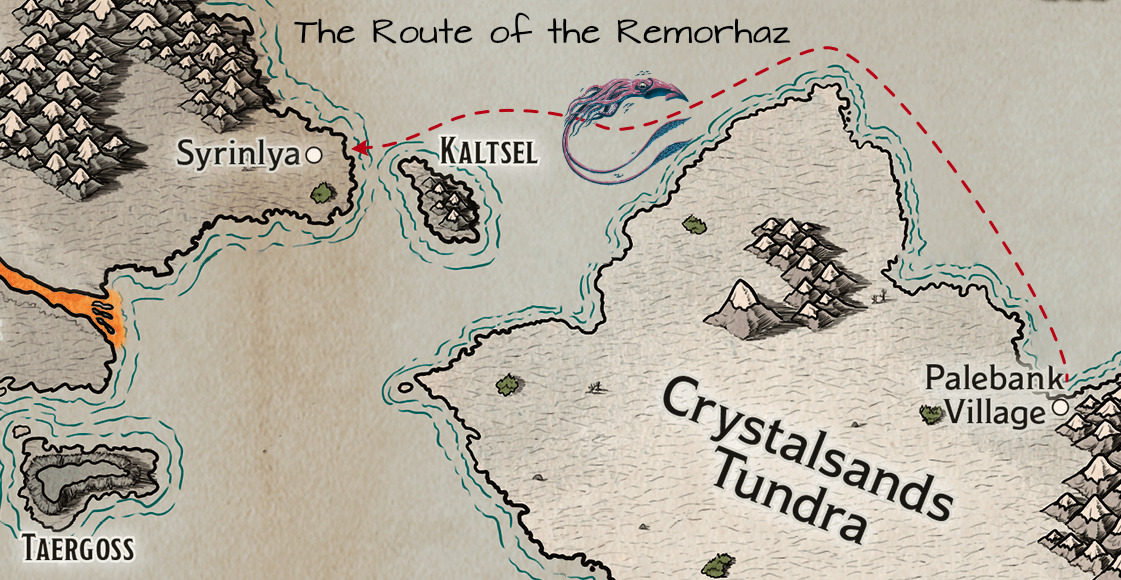
\includegraphics[keepaspectratio]{remorhaz_route.jpg}}
\end{figure*}

``Get ready to aim and fire!'' Captain Stonebeard bellows as he rapidly
reloads the ballista. In that fleeting moment, Doctor Pepe emerges like
a phantom, his crossbow bolt striking true into the squid's vulnerable
flank. The beast roars in pain, its thick, dark flesh quivering from the
impact.

Enraged and wounded, the colossal squid reacts with malignant fury. Its
writhing tentacles thrash through the salt-laden air, and one
particularly vicious limb finds its mark on Elara, ensnaring her. Her
hands clutch at the slick, unyielding surface of the creature. The harp
at her side falls silent as she struggles, caught in the squid's
vice-like grip.

Another abrupt strike from the squid's beak leaves a gaping wound in the
ship's hull. Thick splinters and dislodged timbers bear silent witness
to the beast's brutal might. Amid the clamor of battle, Ingrid's voice
wafts upward from below, barely registering over the cacophony of
combat: ``Are you sure you wouldn't like a sandwich?''

Halite's broad arm hurls a javelin that whistles through the frigid air,
colliding with one of the squid's thick tentacles. The impact
reverberates--- a flash of victory as the creature recoils, wounded by
the force of his strike. At the same moment, Whisper dashes to Elara's
aid. With feline agility, she slashes at the slimy appendage
constricting her, her claws raking into its flesh. A burst of raw
determination follows as she unleashes a flurry of attacks that loosen
the tentacle's grip enough for Elara to breathe, but not enough for her
to escape.

Across the chaotic deck, Ironfist steadies himself and lines up the
ballista, the massive weapon creaking as he aims it squarely at the
disordered beast. Not far away, the wiry wizard, face alight with fervor
and exhaustion, summons a bolt of shimmering blue energy. The air
crackles with ozone as a sustained electric arc connects with the squid,
sapping its monstrous vitality.

Kragor charges, hammer raised high in a wild swing, but his blow misses,
clanging uselessly against the ship's railing. Scarlet seizes the
moment: she maneuvers nimble fingers over the ballista's trigger, and
its bolt flies ahead, striking home into the beast's pulsating flesh
with a resounding crash. Gerhard then finds his focus. His longbow sings
as an arrow arcs through the gloom, finding its target in one of the
squid's unblinking eyes.

Under the relentless assault, the colossal creature falters, its
thrashing slowing until it releases Elara and finally sinks into the
inky depths. After a gasp of relief, Elara calls out over the din to
Ingrid below deck, her voice lilting and defiant, ``Sandwiches for
everyone!'' A surreal endnote to the turmoil--- a promise of warmth and
camaraderie amid the unforgiving cold.

\section{Gerhard}\label{gerhard}

The crew methodically surveys the damage. The squid's beak has carved a
gaping maw in the ship's hull, and the task of repair falls heavily on
the remaining hands.

Whisper, nimble even in the lingering fear, takes to the rigging, aiding
in the salvage operation. She peers into the depths, her vision
unnervingly clear, but the fog obscures the scene.

``Keep wits sharp and hearts steadfast,'' the captain's voice cuts
through the hush aboard the Remorhaz, a floating island of survival. On
decks slick with salt and battle-scraps, weary heroes meet the
newcomers: Gerhard, former captain of the lost ship; Rorik, his young
crewman; and Bret, a passenger.

``Well met,'' Halite says, his voice crisp. ``What brings you so far
out?''

Gerhard, weathered and mid-thirties, steps forward, brown eyes
reflecting relief and deep caution. ``Thank you,'' he breathes, voice
tight with gratitude and disbelief. ``The Frostfang\ldots{} my
ship\ldots{} gone. That squid! I thought I was dead. Ran across the
water, carrying Rorik. This family heirloom saved me.'' He gestures
wildly. ``And that aasimar\ldots{} almost killed! What the hell!''

Rorik, barely seventeen, watches his captain, wide-eyed. Halite,
however, stands rigid, scrutinizing Gerhard. Suspicion cuts sharper than
the chill air; Halite knows survivors don't always bear honest scars.

At the rail, Bret's robed figure steps forward. Kragor recognizes the
sigils: a symbolic design of three inward-pointing diamond shapes with
eight curling spires underneath. This wizard is a member of the Cerberus
Assembly, a powerful conclave of mages in the Dwendalian Empire. The
wizard nods solemnly to Gerhard. ``The sea tests us all,'' Bret intones.
``Perhaps misfortune portends a greater journey.''

Halite's gaze narrows on Gerhard, pressing. ``Specifically, what were
you doing out here?''

Gerhard's breath clouds the frigid air. ``My kin have always plied these
waters. Fishing\ldots{} crabbing, mostly.'' He falters, eyes darting
across the ravaged deck. ``But we found a new source of income. Ferrying
passengers, mostly one way to Eiselcross.'' He gestures toward Bret.
``That mage offered a fortune in gold for his transport there and back
again.''

Bret stands nearby, clearly agitated, his words laced with a demanding
edge. ``I require passage to Icehaven, Captain,'' he declares, his voice
tight with urgency. ``I bear tidings of utmost import. Our vessel is
lost; I must deliver my news without delay. I will provide recompense
for diverting your ship.''

Stonebeard remains unmoved. ``Such a course is impossible,'' he rumbles,
his voice a deep echo of the sea. ``My obligations lie with the
Glassblades; my route must be followed. You may remain aboard. After
completing our appointed rounds, we shall deposit you at Palebank
Village. Another vessel can convey you to Icehaven from there. I am
heartened we rescued you, fortunate you remain living. But expect no
more than offered.'' His gaze fixes upon the traveler with steely
resolve. ``Assist cleaning the foredeck. There is work to be done.''

\section{Land ho}\label{land-ho}

The afternoon fog clings suffocatingly to the Remorhaz, smothering the
sea and reducing the ship to a cautious crawl. In this soup, dead
reckoning is Mera's only guide. Scarlet summons Sparky, her owl
companion, a flash of gold against the gray. ``Fly up, Sparky,'' she
commands, voice tight. ``Find the sun. Tell me how long it takes. And
look for land.''

Sparky beats upward, swallowed instantly by the milky expanse. The crew
watches, hope and anxiety warring on their faces. Three minutes pass.
Four. The wingbeats fade into silence. Five minutes stretch into six,
then seven, then eight.

Suddenly, a spectral shape wheels out of the gray. Sparky circles,
settling onto Scarlet's shoulder. The connection flares, and she sees
through the owl's eyes. ``Took a while to break through,'' Scarlet
reports, her voice hushed, barely carrying over the creak of timbers.
``Up there\ldots{} just clouds. A sea of gray, stretching forever. No
land.''

A small, wry chuckle escapes her. ``Sparky did mention seeing tentacles
in the water, though. Said they smelled bad\ldots{} like farts.''

A collective sigh escapes the crew, a shared breath of weary
disappointment. Hope is a fragile commodity here. The Remorhaz creeps
onward, the search continuing within the fog's suffocating embrace.

The galley bustles with activity, Chef Ingrid impressed with our tale of
the giant squid, her moon-and-rune amulet glinting in the lamplight.
Despite the chaos, a sense of camaraderie pulses through the ship as the
crew gathers--- survivors and newcomers alike.

Kragor, brow furrowed, leans towards the wizard Bret, peppering him with
questions. Bret, clearly burdened by secrets, folds his hands
cautiously. ``I am bound by oaths,'' he states, his tone careful, ``to
maintain discretion regarding my objectives within Eiselcross.'' His
eyes dart around the galley.

Kragor persists. ``But passage to Icehaven? You mentioned tidings of
utmost import. Surely, some details for fellow adventurers?''

Bret sighs, shoulders slumping. ``We uncovered valuable information and
encountered\ldots{} Aeorian constructs in the wastes. It is vital that I
reach Icehaven. And soon.''

``Seen any gold vials?'' Kragor pushes, relentless.

Bret's face remains impassive. ``The antidote for the Frigid Woe?
No.~Fortunately, we did not encounter that dreadful affliction.''

Sensing the rising tension, Elara raises her glass with a bright smile.
``To new beginnings,'' she declares, her voice ringing with cheer, ``and
to surviving giant squids!''

Laughter erupts, instantly easing the weight of suspicion. The crew
celebrates, reveling in their shared survival. Though fog still clings
thick to the Remorhaz outside, a warmth begins to bloom within the ship,
where adventurers share a meal among friends.

Below decks, Ingrid's promised feast wafts upwards--- smoked fish and
steaming bread, a comforting aroma cutting through the lingering brine
and stench left by their monstrous assailant. The three shipwreck
survivors--- Gerhard, Rorik, and Bret--- are formally integrated into
the temporary community forged by shared peril. Gerhard still looks
stunned, his eyes periodically flicking towards the deck as if expecting
the shattered Frostfang to reappear from the mist. Rorik, barely a man
in years, sticks close, while Bret, the wizard, observes the adventurers
with guarded curiosity.

Scarlet approaches Gerhard, her expression sympathetic but gaze direct.
``Gerhard, you said your family sailed these waters long? Your family
name?''

He pulls his attention from the grey void beyond the porthole.
``Eisner,'' he replies, rubbing a hand over his burgeoning beard. ``Of
Icehaven. Fishermen for generations. Crabs, mostly. That boat\ldots{}
she was everything.'' He gestures vaguely towards Rorik. ``My life, his
livelihood\ldots{} gone.'' He sighs, a plume of condensation in the cool
air. ``We'd only recently started ferrying passengers. Trying a new way.
Bret here offered good coin.''

``Is there somewhere\ldots{} we might rest?'' Gerhard asks, looking
towards Captain Stonebeard, who surveys the gathered company, his face
grim but resolute.

``Aye,'' Stonebeard nods curtly. ``Bunks enough. You earned your
place.''

As the survivors find spots at the galley table, laden with Ingrid's
platters, conversation turns to the adventurers' quest. Halite, Kragor,
and Elara briefly explain their mission: the Frigid Woe spreading from
Palebank Village, stolen Aeorian artifacts, Hulil's desperation, and
their current journey to Eiselcross seeking the cure Elro described---
the milky liquid in golden vials. Gerhard and Rorik listen intently,
their own recent brush with death making the tale resonate deeply. Bret
listens too, his face impassive, betraying nothing.

Mera, the navigator, consults her charts, brow furrowed. ``With this fog
and the delay\ldots{} we lost time,'' she announces. ``But if the
weather clears, we could reach Syrinlya by tomorrow afternoon.''

A collective sigh ripples through the crew. Landfall is close.

Dinner is subdued, a recounting of the battle punctuated by shared
relief. Later, mugs refilled, Elara retrieves her harp. Small against
the vast, fog-bound sea, the instrument sings under her fingers, a
melody of quiet longing and resilient hope filling the galley. The notes
hang, fragile beauty against their harsh reality. Even Bret seems
softened, gaze distant. When the song ends, respectful silence yields to
appreciative murmurs.

As evening deepens, the ship's routine returns. Watches are assigned:
Scarlet first, senses alert to wind and timber, Sparky a silent,
feathered presence beside her. Whisper follows, melting into deck
shadows, eyes piercing the gloom. Gerhard takes the third watch,
grateful for the normalcy. Captain Stonebeard joins him near the helm,
leaning on the rail, fog swirling like ghosts.

``Sorry about your vessel, Gerhard,'' Stonebeard says, voice low. ``Hard
thing, losing your ship.''

Gerhard nods, staring into the white abyss. ``Aye. Good boat. Fast. Grew
up on her. Dad taught me fishing there.'' He pauses. ``Good thing I have
insurance.''

Stonebeard raises an eyebrow. ``Insurance?''

``Aye. Have you never found a wizard willing to take a few gold a month
against the value of your hull? Got a good rate from an Empire fellow.
If she sinks, he buys me a new one. Family's done it a long time.'' He
shrugs. ``Still\ldots{} devastating. But we're not bankrupt.''

Stonebeard grunts, filing the information away. ``Boats are expensive.
Taken many voyages myself.'' He shifts his weight. ``Given the
circumstances, saving your lives, there's no charge for passage to
Palebank Village.''

Gerhard turns, surprise, perhaps offense, flickering in his eyes. ``No
charge? Captain, with respect, that's naval etiquette. Rescued souls
aren't passengers for fare.''

Stonebeard meets his gaze steadily. ``My apologies. Correct, of course.
Force of habit.'' He sighs wearily. ``Long few days.'' He gestures
vaguely below deck towards where Bret presumably sleeps. ``That
squid\ldots{} seemed focused. Like it was after your passenger.''

Gerhard shivers, though perhaps not entirely from the cold. ``Never seen
the like. Thirty years sailing these waters. Seen krakens, sure. But
never one going after a ship, after someone, like that. Not even for a
hold full of my crabs.''

The two captains stand silent awhile, solitary figures keeping vigil
against the vast, uncaring sea and spectral fog.

Elara takes the fourth watch, relieving Gerhard. Settling near the bow,
harp resting beside her, she resolves to stay alert, but the battle, the
song, the journey's weight\ldots{} it all presses down. The rhythmic
slap of waves against the hull becomes a lullaby. Her eyelids grow
heavy. One moment she scans the impenetrable white wall ahead; the
next\ldots{}

She jerks awake with a start. Grey dawn light filters through thinning
fog. Guilt floods her--- she slept. Heart pounding, she scrambles up,
frantically scanning the deck, the sea. Nothing. No alarms, no
disturbances. The Remorhaz sails on, undisturbed. Relief wars with
embarrassment; apparently, the Frigid Depths granted her unguarded
peace.

As the morning progresses, the pale sun burns away the fog. By noon,
visibility stretches for ten miles across choppy, grey-green waves under
a brightening sky. And there, rising from the sea to the south, is the
unmistakable shape of land--- jagged, snow-dusted peaks against the
horizon.

A shout goes up from the crow's nest, echoed by murmurs on deck. Captain
Stonebeard strides to the railing, squinting. A rare grin splits his
beard. ``Ah, Kaltsel to the south!'' After a brief conference with the
navigator, he adds ``Mera puts us two hours out from Syrinlya!'' He
turns, voice booming across the deck, energized. ``Alright, you lot!
Look alive! Pack your gear and prepare for landfall! The Frigid Depths
haven't beaten us yet!''

The salt spray now freezes almost instantly upon hitting the deck. Since
leaving Palebank Village, the world has steadily bled color and warmth,
surrendering to an encroaching reign of ice. The air bites with a
ferocity that makes the fog-chilled waters seem almost temperate by
comparison. Under the finally clear, brittle sky, the Remorhaz glides
towards a coastline that looks like the jagged teeth of some immense,
frost-covered beast, its peaks clawing at the sky.

Mera's calculations prove precise. As the sun begins its slow descent,
casting long, pale shadows across the waves, the ramshackle outpost of
Syrinlya comes into view. It's less a town and more a temporary scar
upon the landscape--- a sprawling camp of fur-lined yurts huddled
against the relentless wind, smoke whipping horizontally from their
capped peaks. Figures bundled against the cold--- mostly dwarves and
elves, judging by their builds--- move between the structures.

Stonebeard brings the Remorhaz expertly alongside a crude dock fashioned
from timber and ice. ``Alright, Syrinlya!'' he bellows, his voice
carrying over the wind's howl. ``We'll unload cargo, then take on
whatever's heading back south. We depart for Palebank Village in three
days. Plenty of time for you lot to find your contact.'' He gives a curt
nod to the adventurers. ``Mind the ice.''

\section{Syrinlya}\label{syrinlya}

The wind assaults the party as they step onto frozen ground, driving
needles of snow into exposed skin. Kragor pulls his cloak tighter,
muttering about unnatural cold. A stout, weathered dwarf woman with a
wild mane of shaggy grey hair approaches, stamping heavily booted feet.

``Morgo Delwur, at yer service!'' she declares, her voice rasping
through the gale. ``Heard you were comin'. Lookin' for Orvo Mustave?''
She gestures vaguely inland. ``His yurt's over there. And the Buyer?''
She points to a larger, well-maintained yurt. ``That's his place.
Fancy.''

She sweeps an arm around the disparate groups of adventurers milling
about near sputtering fires. ``Everyone's here for the same thing, eh?
Aeorian treasure. Big risks, big rewards\ldots{} or just frozen toes.''

Halite asks, ``Can you point us towards provisions? Snowshoes,
perhaps?''

Morgo nods. ``Aye, plenty o' folk lookin' to sell you gear. Some make
more coin tradin' than diggin'. Follow me.'' She leads them through the
camp to another large, fur-lined yurt. ``You can bunk here. Belonged to
some rich elf lordling. Came lookin' for adventure, poor sod. Got
himself eaten by a sabre-tooth tiger his first day out.''

Scarlet's eyes widen. ``In the yurt?!''

``Gods, no, lass!'' Morgo barks a laugh. ``We don't let the big cats
wander camp! Nah, he went out, didn't listen to his guides. They found
his boots and\ldots{} well, not much else. His loss, your gain.''

Inside, the yurt is surprisingly spacious and less frigid. A stone fire
pit sits centrally; thick, fur-lined hammocks hang from sturdy poles.
``Right then,'' Scarlet steps to the pit, whispers an incantation. A
small flame springs to life, instantly pushing back the chill.

Gerhard, utterly lost and overwhelmed, drifts away from the nascent
fire, staring blankly at a fur-lined wall. Elara approaches the bereaved
captain. ``Gerhard,'' she says softly, her voice warm despite the chill.
``It's\ldots{} a lot to take in. But you're safe now.''

Scarlet steps closer to the crackling flames. ``She's right. You
survived something terrible. You're stronger than you think. And you're
welcome here.''

He manages a weak, haunted smile. ``Thank you\ldots{} my boat\ldots{}
everything\ldots{}'' Rubbing his face, he trails off. ``I\ldots{} I
think I need rest.'' He finds an unoccupied hammock and climbs in,
pulling a fur blanket over himself.

While Gerhard settles, Kragor spots an open wooden crate. Curiosity
piqued, he investigates. Inside lies a trove: weeks of trail rations,
fifty feet of fine silk rope, a thick woolen blanket, another grappling
hook, a sturdy miner's pick, and, tucked beneath it all, a small,
leather-bound book.

Kragor picks it up. The gold-leaf title reads: ``Adventure Sexy: Impress
Potential Lovers with Great Deeds'', by Scanlan Shorthalt.

He grunts, holding it aloft. ``Looks like our elf wasn't just after
treasure.''

Elara peers at it. ``Oh, Scanlan again. So popular\ldots{} I'll have a
following like that someday.'' She winks.

Whisper sniffs disdainfully. ``More useful than poetry, perhaps,'' she
eyes the silk rope with interest.

``Miner's pick?'' Halite rumbles, taking the tool from the crate and
testing its weight. ``Could be useful.''

Morgo nods at the fire. ``Right then. Shelter's sorted. Provisions are
sold near The Buyer's place. Meself, I'll be heading on an expedition
west tomorrow.'' She cracks her knuckles. ``Any final questions?''

``Thank you for your hospitality, Morgo,'' Halite says with a respectful
nod.

``Aye, thanks for the yurt,'' Kragor adds, tossing the Scanlan Shorthalt
book dismissively into its crate. Elara quickly retrieves it with a
thoughtful hum.

Morgo gives them a final nod. ``Stay warm. Stay sharp. Don't get
eaten.'' She turns and vanishes into the swirling snow.

Inside the yurt, the fire crackles against the wind's mournful
Eiselcross howl. It's late afternoon, their fifth day since leaving
Palebank Village. Syrinlya is harsh, potentially deadly, but they have
shelter, supplies, and a lead.

\section{Orvo}\label{orvo}

``Alright,'' Halite says, hefting the miner's pick. ``Let's find this
Orvo Mustave. Then we'll see about snowshoes and other provisions.''

Whisper interjects, ``It's getting late. Best split up: some get
supplies, others find Orvo.''

They agree. Whisper, Scarlet, and Doctor Pepe head for the provision
yurts near The Buyer's large dwelling, the spot Morgo indicated. Wind
tugs their cloaks as they navigate snow-dusted paths between structures.

Meanwhile, Kragor, Halite, Elara, and a subdued Gerhard seek Orvo
Mustave's yurt. They find it slightly apart, smaller than theirs, smoke
rising bravely against the grey sky. Before it, a modest campfire
struggles against the cold. A young dwarf sits beside the flames,
shortsword across his lap. His dark, relatively short beard frames a
face marked by a prominent scar--- three ragged lines, like a claw mark
dragged across his cheek. He looks up as they approach, warming his
hands.

``Oh, hey,'' he calls out, his voice rough but friendly enough. ``How
y'all doing?''

Halite steps forward, his bulk casting a long shadow in the afternoon
light. ``Well met. We seek Orvo Mustave. Elro of the Glassblades sent us
from Palebank Village.''

The dwarf nods, pushing himself up slightly from his resting spot. ``I'm
Orvo. Elro sent word you'd be coming. Heard you came with the
Remorhaz.'' He squints at the disparate group before him. ``Quite the
collection. Where are you folks from?''

Kragor pulls his cloak tighter against the wind whipping off the ice.
``Bladegarden.''

Orvo whistles softly. ``Bladegarden? Long way. Caught between the Empire
and the Dynasty there, eh?''

Halite gestures vaguely south. ``The Menagerie Coast is my home.''

``Ah, the Menagerie,'' Orvo nods. ``Heard it's warmer.'' He turns his
gaze to Elara, who beams, her celestial heritage almost palpable even
bundled in furs. ``And you, lass?''

Elara steps forward, eyes sparkling like distant stars. ``Me? Oh, I'm
from the stars! Just landed here recently.''

Orvo blinks, then chuckles, a low rumble in his chest. ``From the stars,
eh? Okay then. That's\ldots{} different. Welcome to Syrinlya,
Star-Lass.'' His gaze shifts to Gerhard, who seems braced for the
attention.

Gerhard clears his throat, his voice quiet, almost rough from disuse or
emotion. ``Gerhard Eisner. My family\ldots{} we're from the Greying
Wildlands, north of the Empire. We\ldots{} fished these waters.
Generations of us.'' He gestures vaguely out towards the frozen sea, his
expression momentarily shadowed by unspoken loss.

Orvo nods slowly, his expression softening with understanding. ``Greying
Wildlands? Know the coast. Tough folk live up there. And fishing these
waters\ldots{} takes grit.'' Sensing Gerhard's recent hardship, he
doesn't press, turning back to the group. ``Well, welcome to Syrinlya.
You all came a long way. What can I do for you? Elro's message just said
you were looking for something.''

Elara clasps her hands together. ``We are on a quest! A most urgent one.
We seek\ldots{} a cure! A milky liquid, held within vials of gold. Have
you seen such wonders?''

Orvo scratches his scarred cheek, looking genuinely puzzled. ``Gold
vials? Milky liquid? Can't say I have. Sounds fancy.''

``Familiar with the Frigid Woe?'' Halite asks directly, his tone sharp.
``The freezing sickness?''

Orvo's expression darkens. ``Aye. Nasty business. Came across
the\ldots{} source material\ldots{} out with Urgon.'' He pauses, brow
furrowed. ``Wait, you know Urgon? My buddy?''

Kragor steps forward, switching smoothly to Dwarvish, his voice low and
somber. ``Orvo\ldots{} we have bad news about Urgon.''

Orvo's eyes widen slightly. ``Bad news? What\ldots{} what happened?''

``He contracted the Frigid Woe,'' Kragor states plainly. ``From one of
the blue vials you recovered. He\ldots{} did not survive. Died back in
Palebank Village.''

The dwarf stares, comprehension dawning slowly. His gaze drops to the
struggling fire; he kicks absently at a chunk of ice near his boot.
``Ah, hells. Urgon\ldots{}'' He shakes his head, the movement sluggish
with disbelief. ``Damn it. Knew that stuff was dangerous. He\ldots{}
could be a real jerk, but\ldots{} he was my mate.'' Looking up, grief
and anger cloud his eyes. He switches back to Common, his voice thick.
``That bloody sickness. Did\ldots{} did you handle those blue vials?''

``We secured the ones Hulil Lutan had,'' Halite confirms. ``She got them
from Urgon, it seems. Did you keep any?''

Orvo shakes his head again. ``Nah. Sold my share to The Buyer right
after the dig. Needed coin. Told Urgon to be careful.'' He sighs, a
ragged sound. ``So the cure\ldots{} the gold vials you're after\ldots{}
you think they're out where we found the blue ones?''

``Elro believes so,'' Elara confirms urgently. ``Where did you find
them, Orvo? People are still sick back in Palebank Village.''

``Right, right.'' Orvo gathers his thoughts. ``The place is called
Salsvault.'' He gestures northwest. ``About two hundred miles that way,
in the Thin Sheets. The ice there gets treacherous, shifting. The ruin
itself is\ldots{} odd. Better shape than most. Feels like something's
holding it together, maybe magic from the city's fall.''

``Two hundred miles?'' Kragor's brow creases as he calculates. ``How
long does that take?''

``Depends on your pace,'' Orvo replies. ``Normal speed, maybe eight or
nine days--- twenty-four miles a day, give or take. Push it to thirty,
but you risk exhaustion. Or slow it down, safer at eighteen miles a day,
easier to spot trouble.'' He rubs his hands near the fire. ``Trouble
like the Ice Mephits. Elemental pests drawn to the magic keeping the
place intact.''

``Mephits?'' Elara asks, intrigued. ``Are they aggressive?''

``Oh aye,'' Orvo nods grimly. ``Saw a few lurking outside. We thought we
were clever sneaking past them. The real trouble was inside. Looked like
a lab. We barely made it into the third chamber before these animated
suits of armor came alive and chased us out. Not as big as you,'' he
glances at Halite, ``but still big enough. We snatched what we could---
the vials and a few other bits--- and didn't look back.''

``So you didn't find any gold vials?'' Halite presses.

``Nah. Didn't know what the blue ones held then, just that they seemed
valuable.'' Orvo sighs, regret heavy in his voice. ``Poor Urgon. If I'd
known\ldots{}''

``Is there no faster way to Salsvault?'' Kragor asks. ``Horses? Sled
dogs?''

Orvo snorts. ``Horses? They'd freeze or break a leg in an hour. Dogs,
maybe, if you find a trained team willing to risk it. Most folks stick
to snowshoes. Best bet, really.''

``Where can we acquire those?'' Halite asks.

``No proper shops here,'' Orvo confirms. ``It's all trade and salvage.
Folks pick gear off expeditions that\ldots{} don't come back complete.
Try asking around near The Buyer's yurt. Fellow named Javel, might have
some. Three yurts over from the big one, towards the ice cliffs. But
expect to pay. Supply and demand, eh? Probably run you two gold a pair,
maybe more if he thinks you're desperate.''

As Orvo finishes speaking, the rest of the party approaches, emerging
from the maze of yurts. Scarlet brushes snow from her cloak, Whisper
moves with silent steps, and Doctor Pepe offers a curt nod.

``We struck out on supplies,'' Scarlet admits reluctantly. ``However!''
she holds up a small, grease-stained paper bag. ``Scones. Apparently,
someone here bakes.''

Doctor Pepe eyes the bag. ``Are they gluten-free?''

``They're squid-based,'' Whisper announces, her voice flat but her eyes
betraying an eagerness to try them.

Orvo looks between the two groups, then back towards the bleak, frozen
wilderness stretching away to the northwest. ``Right then. Looks like
you're all set to talk gear. Salsvault ain't goin' anywhere. But those
suits of armor\ldots{} watch yourselves. They freaked me right out.'' He
gives them a final, weary nod. ``Good luck. Hope you find what you're
lookin' for. For Urgon's sake, too.''

The wind howls a dirge through Syrinlya's haphazard sprawl of yurts as
the reunited party stands outside Orvo Mustave's modest dwelling. The
dwarf offers a weary nod before retreating to the warmth of his fire,
leaving the adventurers to the biting cold. Snow swirls around their
boots, stinging exposed cheeks.

\section{Javel}\label{javel}

``Right,'' Halite rumbles. ``Snowshoes. Orvo mentioned a trader named
Javel, three yurts over from The Buyer's place.''

Whisper nods, her tail twitching beneath her cloak. ``Near the ice
cliffs. Let's not waste time.''

They trudge through the deepening snow, the crunch of their boots
muffled by the wind. Bundled figures pass by, faces obscured by scarves,
gazes cast downward against the elements. The air smells sharp and cold.
Gerhard follows silently, haunted by memories of his lost ship.

Following Orvo's directions, they locate the specified yurt---a larger
structure with smoke curling from its central vent. A rough-hewn sign
hangs beside the entrance, depicting a crossed pickaxe and snowshoe.

Elara, ever the diplomat, pushes the flap aside and steps inside, the
others close behind. The immediate change is palpable; the wind's roar
diminishes, and though the air is cold, it lacks the vicious bite of
outside. The interior is cluttered yet organized, filled with furs,
ropes, and adventuring gear. Near a sputtering fire pit sits a dwarf so
ancient his braided beard pools around his feet. He looks up, watery
eyes blinking in the gloom, and lets out a series of rattling coughs.

``Good day, Master Dwarf! I've heard good things about your shop.''
Elara chirps, her voice bright in the dim, smoky yurt. She steps
forward, radiating warmth despite the chill. The old dwarf squints at
her.

``Eh? What's this now?'' he rasps. ``Well now\ldots{} yer a sight. What
in the Nine Hells are ya? Is that\ldots{} a horn on yer head?''

Elara smiles, a dimple appearing in her cheek. ``Some say it's horny.''

The dwarf lets out a wheezing cough that could be a chuckle. ``Heh. What
can I do for ya?''

``We're new here,'' Elara says, pulling a small, worn leather-bound book
from her pack. ``Hoping you might help us. By the way, your cough sounds
dreadful. I don't have any herbs, but I find this book helps
during\ldots{} downtime.'' She offers it to him.

The dwarf's eyes widen slightly as he takes the book with a trembling
hand. ``Tusk Love? Gods\ldots{} have ya read Chapter Three?''

``Oh, it was so good,'' Elara gushes, clasping her hands. ``The size of
those hands! And the tentacles! My horn was horny when I read that
chapter!''

``Aye!'' The dwarf nods vigorously, another cough rattling him. ``Best
thing to read when yer laid up. Just lay back and read Tusk Love.'' He
sets the book aside and pulls out a long pipe, tamping something into
the bowl. ``A woman after me own heart. So, what brings this fine
company to ol' Javel's Emporium? I'd guess me boyish good looks, or yer
lookin' for gear.''

``Well,'' Elara leans in conspiratorially, ``we definitely noticed the
boyish good looks.''

``Ho ho!'' Javel chuckles, a sound like rocks tumbling. ``Yer not wrong
there! But I suspect gear's the main order o' business. What do ye need?
Snowshoes?''

``Indeed,'' Halite confirms. ``Seven pairs. We're on an urgent
mission---to stop a\ldots{} popsicle sickness.''

Javel raises an eyebrow. ``Popsicle sickness? Ah, the Frigid Woe. Nasty
business. Commendable you want to stop it.'' He studies the party.
``Goliath, Tabaxi, Orc, Halfling\ldots{} you lot come in all shapes, eh?
Let me see what I got.'' With a groan, he rises, his beard trailing the
packed-earth floor, and disappears into the shadows of the yurt.

They hear him muttering, coughing, and the unmistakable shuffle of gear,
occasionally interrupted by a clatter and a dwarven curse. Halite shifts
his weight, scanning the yurt's contents. His thoughts drift beyond the
immediate dangers of Salsvault--- Eiselcross, Aeor\ldots{} ancient
magic, lost knowledge. Perhaps there are secrets here beyond just a
cure. A seed of ambition takes root: survive this, find the cure, yes,
but also learn. Bring back more than just stories to his people.

Javel reappears, dragging several pairs of snowshoes. ``Right then. Got
yer sizes, I reckon.'' He sorts through them. ``Goliath\ldots{} these'll
do.'' He tosses a large pair towards Halite. ``Orc, Tabaxi, the rest of
ya. Oh and erm, Halfling\ldots{}'' He pauses, holding up a pair stained
dark red. He glances at Scarlet. ``Yours\ldots{} uh\ldots{} well,
they're red. Ignore that.''

He piles the seven pairs together. ``Normally, fifteen gold for the lot.
But\ldots{} I like yer horn, lass. And yer taste in literature.'' He
winks at Elara. ``Twelve gold pieces for the lot. That's like getting
three pairs free, considerin' the goliath tax.''

``How about ten gold?'' Elara counters smoothly. ``Chapter Eight was
quite illuminating. Those pixies! Glitter me, that's all I have to
say.''

Javel strokes his beard, considering. Elara beams hopefully. He shakes
his head. ``Twelve's fair. But\ldots{} seein' as yer on a noble
quest\ldots{}'' He rummages behind a pile of furs. ``I'll throw in these
four ice hammers \ldots{} and,'' he holds up a finger indicating a
pause, and rummages around. He then produces a few sturdy climbing
hammers along with a quartet of waxed leather pouches, each roughly the
size of a grown man's fist. ``\ldots{} Oil. That's a whole lot--- seven
pairs o' shoes, four hammers, four pounds of oil--- thirteen gold
pieces. Final offer. Won't find better in Syrinlya, guaranteed.''

Scarlet steps closer, eyeing the red snowshoes Javel set aside. In
Dwarvish, she asks, ``Why are the snowshoes red?''

Javel leans in, lowering his voice. ``Ah. Pre-owned, ye see. Prime
condition, but\ldots{} belonged to a halfling.''

``And the color?'' Kragor interjects.

Javel glances at the yurt flap, conspiratorial. ``Keep yer eyes open for
Yetis out there.''

``Are they partial to halflings?'' Scarlet asks dryly.

``Depends how hungry they are,'' Javel grunts. ``But the red\ldots{}
aye. That's bloodstain. Couldn't quite scrub it all out.''

Nearby, Gerhard listens in on the Dwarvish conversation, and summarizes
for Halite in a murmur, ``Sounds like a Yeti ate the last owner.''

Scarlet inspects the snowshoes more closely. Years of reading nature's
signs allow her to identify the stains with chilling certainty. It's old
blood, soaked deep into the hide. She wrinkles her nose but nods.
``They'll do. Thirteen gold.''

As the party pools their coins, Javel grunts with satisfaction, tucking
the gold into a pouch. ``Pleasure doin' business with ya.'' He reaches
under some furs and pulls out a dusty bottle of amber liquid. ``And
before ye go\ldots{} welcome to Syrinlya.'' He hands it to Elara. ``On
the house. Sandkeg's High. Not the fancy stuff, but it'll warm yer
bones.''

``Why thank you, generous soul!'' Elara replies, taking the whiskey.

``Right then,'' Kragor says, eyeing the bottle. ``After fighting a giant
squid and learning we're facing an eight-day trek through Yeti
territory, I think a drink's in order.''

``Agreed,'' Halite nods. ``Let's head back to the yurt. We need to
plan.''

They thank Javel and step out into the relentless wind, clutching their
new gear. The evening sky darkens, the cold deepening as the prospect of
their journey looms large. Back at the elf-lord's abandoned yurt, with
Gerhard huddled miserably in a hammock and the whiskey making the
rounds, they face the stark reality of Eiselcross. They have gear and a
destination, but the path ahead is long, cold, and fraught with unknown
perils.

\chapter{Intermission}\label{intermission}

The yurt's interior glows with a warm, flickering light from the central
fire pit, a defiant warmth against the relentless Syrinlya wind that
howls outside like a wounded beast. Doctor Pepe is the first to notice a
message from Captain Stonebeard left on the yurt's only table: the
Remorhaz requires weeks of repair before it might be able to make
another crossing of the Frigid Depths. The clock ticks mercilessly for
the Liel-Tethwick family, with Salsvault 200 miles away and the Frigid
Woe's icy grip threatening to claim their lives. It had already been
five days since they had left Palebank Village, and the adventurers knew
that they must set out immediately.

Elara, her celestial nature radiating with optimism, sets about lifting
their spirits. Her hand drum sets a vibrant rhythm, a defiant heartbeat
against the wind's relentless howl. Her eyes gleam with an almost manic
energy as she launches into a quick, lively beat.

Gerhard sits hunched, a man broken by loss. The \emph{Frostfang}, his
life's work, now exists only in memory. Rorik's placement aboard the
Remorhaz feels like salt in an open wound. ``What's-his-name is dead to
me,'' he mutters, his voice cracking with unshed grief, whisky sloshing
in a trembling hand.

Scarlet moves closer, her presence as grounding as the earth itself.
``Even after the fiercest blizzard, the smallest shoot can still find
the sun. Even when the great beasts tear through the forest, life finds
a way to grow back, sometimes stronger, sometimes in a new and
unexpected form,'' she says to Gerhard. ``You've lost much, yes, but
you're still here. And your skills, your knowledge of this unforgiving
land\ldots{} they're not lost. They're waiting. Our quest isn't just for
some glittering bauble, though treasure does have its uses. We're
seeking a cure, a way to mend what's broken in the world, much like you
might one day find a way to mend the loss within you.''

Her words are a balm, cutting through Gerhard's fog of despair. He looks
up, really sees the faces around him for the first time. Something
shifts in his eyes--- a spark of possibility rekindling. Finally, he
lets out a shaky sigh. ``Well, what the hell. There's really nothing I
can do, stranded here with no boat and no crew. I might as well go with
you lot. May I find a fortune while keeping you out of trouble.''

Halite claps him on the back, the impact nearly knocking Gerhard off
balance. ``Welcome aboard,'' he rumbles with a genuine smile. Whisper
offers a small, encouraging nod. The others add words of encouragement
as well, all of them welcoming the skills Gerhard brings to the team.

Elara, sensing the shift in mood, launches into a rambunctious rendition
of ``A Troll's Grin and a Fairy's Hand,'' her hand drum accompanying her
voice as she celebrates their new collaboration. Her lilting song fills
the yurt, promising adventure and companionship, drowning out the wind's
mournful song.

\section{Kragor speaks up}\label{kragor-speaks-up}

Kragor has remained uncharacteristically silent, lost in thought.
Subdued. But as Elara's last note fades, he abruptly stands. He draws a
deep breath, his chest visibly expanding.

``Alright. Listen up. I got something to say,'' he begins, his voice
raw, almost hesitant. He begins the story of his initiation into the
arcane, and as the party leans in, the walls of the yurt seem to melt
away, replaced by the cold, dark streets of Bladegarden.

``I've made it no secret that I get my magic from \ldots{} somewhere
from without our realm. But I never told you how, or why I came here. To
the north. My business is my own. Yet now\ldots{} things are getting
weird. Bad weird. And I fear keeping secrets too close might bring you
to your doom. And then I die too, 'cause we're stuck together now.''

He stares beyond the yurt's walls, his eyes unfocused, lost in a memory
that transcends time and space. He shares the story of the past, and, as
he does, his listeners are able to see the world in the same bleak way
that he does.

``My journey began after many, many moons of strange sleep as I lived on
the streets of Bladegarden. Hearing whispers. Bad dreams full of dark
shapes that called my name. Visions of stars falling, and huge dark
shapes just beyond reach. And something there, watching. Always
watching.'' He pauses, as if trying to grasp the memories. ``Then, on a
very dark night, some man-whelps tried to kill me. But I refused to die
like a nobody. Just another forgotten orc, fatherless trash. I was
scared and nearly dead. So I yelled into darkness\ldots{} I gave up
to\ldots{} whatever the watcher was.''

His eyes blaze with an inner fire as he describes the moment of
transformation. ``Then I felt it!'' he says. ``Cold like night
but\ldots{} nice. It wrapped around me like black smoke. It whispered
secrets in a strange tongue I do not know. Then, power filled me! A war
hammer appeared in my fist from nowhere. I felt no remorse when I
smashed in my attacker's stupid face right then and there, then blasted
the other scum with dark crackling magic that sent them running like
scared rabbits.''

Whisper glances at Halite, a silent question in her eyes: ``Where is
this going?''

Kragor's eyes harden as he adds, ``But I know such magic comes at a
cost. The dreams kept coming, mostly nonsensical. Gradually, they formed
some thought--- a command and a promise for greater power. `Go north.
Cross the frozen north. To Eiselcross.' Don't know why exactly. Maybe to
find something. Maybe to smash something.

``But comrades\ldots{} I've new dreams now. Worse dreams. More than
dreams.'' The orc shifts uneasily from one foot to another, a gesture of
worry that his companions are not used to seeing. ``Back at that tavern,
the Jolly Dwarf, some night I slept bad. Couldn't remember what I
dreamed, but when I woke up\ldots{} my fingers had dirt under the nails.
Broken nails. It made no senses! I am clean \ldots{} fastidious! And
then on the Remorhaz, while crossing the ice sea, I woke up in the
night. But I was not in my bed! I was\ldots{} somewhere else. Couldn't
move. Felt like mountains of ice pressing down on me. Hearing ice
cracking. For a long time, I couldn't even feel myself breathing.
Couldn't scream. This was no dream. It felt like I was locked away,
buried under ice. Then, snap! Back in my bunk. And again, dirt under my
nails! Dirt that should not be there\ldots{} could not be there!''

Kragor shudders, a chill running down his spine that has nothing to do
with the icy wind. ``Whatever got its claws in me\ldots{} it's doing
something with my body when I'm sleeping. And that ain't good for any of
us.''

As Kragor's story ends, a stillness falls over the yurt as the
companions ponder the implications.

Elara is the first to break the silence, her voice soft but resolute.
``We should stay close,'' she says, looking directly at Kragor. ``I'll
bunk near you, keep watch. Maybe we can understand what's happening.''

Whisper's tail twitches nervously. ``Tie him up?'' she suggests, her
feline eyes narrowing.

``No,'' Halite rumbles, shaking his head. ``We may need Kragor's powers
if we encounter trouble. Restraints could slow us down.''

Doctor Pepe leans forward, stroking his chin. ``Interesting predicament.
Sounds like a magical possession, or perhaps something more sinister.''

Scarlet closes her eyes, communing silently with the natural energies
around them. ``There's something\ldots{} off. A presence. But I can't
quite identify it.''

As the discussion continues, Elara retrieves her harp. Her fingers dance
across the strings, weaving a gentle lullaby that seems to soften the
harsh edges of their conversation. The melody speaks of protection, of
peaceful rest, of guardianship against unknown threats.

Gerhard, still haunted but feeling more connected to the group,
volunteers for first watch. The night passes quietly, save for the
discovery that someone in the group snores with the thunderous intensity
of a winter storm.

Halite takes the second watch. The camp remains still, with occasional
sounds of people moving to relieve themselves against the bitter cold.
The wind whispers secrets outside, but nothing disturbs their rest.

Elara's watch is marked by intense focus. Her eyes never leave Kragor,
watching for any sign of movement, any hint of the strange nocturnal
activity he described. But the orc remains motionless, his breathing
steady and deep.

As Scarlet takes the final watch, the first hints of dawn begin to paint
the sky. The sounds of the camp slowly come to life--- the rustling of
sleeping bags, the soft clanking of cooking utensils, the preparatory
movements of travelers readying for a day's journey.

Morning arrives, and Kragor's nails are clean. No mud, no dirt---
nothing to suggest mysterious events.

\section{The Journey Begins}\label{the-journey-begins}

The party decides on a measured pace, hoping to cover approximately 24
miles each day without undue risk. Gerhard, drawing on years of
wilderness experience, prepares their rations. His hands move with
practiced efficiency,

Scarlet sends Sparky, her faithful owl companion, to scout ahead. But
the bird, more accustomed to wooded landscapes, seems perplexed by the
endless expanse of snow. There are no trees, no rocks--- just an
infinite white canvas stretching to the horizon.

As night falls, they make camp beneath a half-moon of Catha, the Moon
Weaver. Ruidus, the small moon, hangs full--- a celestial harbinger of
ill tidings that sends a collective shiver through the group.

During Whisper's watch, a bright light streaks across the sky from east
to west. She makes note of it but waits until morning to mention the
anomaly.

The second day out from Syrinlya brings challenges. A steep cliff face
looms before them, its icy surface treacherous and unforgiving. Halite
steps forward, his massive frame a testament to strength and
determination as he swings the grappling hook up and over the edge of
the cliff. With the grappling hook secured, he scales the cliff with
surprising grace, creating a lifeline for his companions. One by one,
they traverse the obstacle, each movement calculated and precise.

As evening approaches, clouds gather, muting the landscape into shades
of gray and white. The cold is relentless, but they sleep soundly---
except for one.

During her watch, Elara notices Kragor's restlessness. He curls into a
tight ball, his massive frame seeming to shrink. Unable to wake him, she
watches him intentently as he oscillates between struggle and paralysis.
When morning finally comes, his fingernails are once again caked with
mud--- impossible in this frozen wasteland of ice and snow.

On the third day, as they trudge forward, the monotonous white landscape
is interrupted by two rock formations, standing like silent sentinels
approximately ten feet tall. Their sudden appearance is both a relief
and a source of renewed tension, breaking the endless white with their
dark, weathered surfaces.

Something is watching. Something is waiting.

\chapter{Appendix A --- Party
Inventory}\label{appendix-a-party-inventory}

\begin{DndTable}[header=Purse]{Xr}
\textbf{Currency} & \textbf{Amount} \\
Gold & 1,004 \\
Electrum & 18 \\
Silver & 166 \\
Copper & 36
\end{DndTable}

\begin{DndTable}[header=Inventory Adjustments]{XX}
\textbf{Who} & \textbf{What} \\
Doctor Pepe & 130 crossbow bolts \\
Doctor Pepe & Aeorian Dagger, +1 \\
Doctor Pepe & Cook’s utensils \\
Doctor Pepe & Grappling hook \\
Doctor Pepe & Ice hammer \\
Doctor Pepe & Olive drab deerstalker \\
Doctor Pepe & Snowshoes \\
Gerhard & Ice hammer \\
Gerhard & Snowshoes \\
Halite & Cook’s utensils \\
Halite & Miner’s Pick \\
Halite & Snowshoes \\
Halite & one javelin lost while fighting squid \\
Scarlet & Snowshoes \\
Whisper & 50 feet of silk rope \\
Whisper & Ice hammer \\
Whisper & Snowshoes \\
Whisper & one javelin lost while fighting squid \\
Whisper & Oil (4 lbs)
\end{DndTable}

\begin{DndTable}[header=Equipment]{rX}
\textbf{Count} & \textbf{Item} \\
1 & Bottle of Bald Dwarf \\
1 & Gilded Scroll Case \\
1 & Jade Statuette of a Storm Giant \\
1 & Journal of Hulil Lutan \\
1 & Silver Ring (50gp) \\
2 & Potions of Healing \\
3 & months of provisions
\end{DndTable}

{\emph{Book, uncommon}}

Penned by the illustrious, if not always entirely humble, bard Scanlan
Shorthalt, this exquisite leather-bound tome with its full title
``Adventure Sexy: Impress Potential Lovers with Great Deeds'' emblazoned
in glittering gold leaf is less a guide to genuine heroism and more a
compendium of dramatically (and often exaggerated) retold exploits,
carefully curated for maximum romantic appeal.

While it contains questionable advice on actual adventuring, ``Adventure
Sexy'' is filled with Scanlan's unique brand of bravado, wit, and
selective memory, offering numerous examples of how to creatively (and
sometimes stretching the truth) present one's deeds to potential
romantic interests. It's more a testament to Scanlan's ego and
showmanship than a source of arcane power.

{\emph{Weapon, uncommon}}

A finely wrought dagger previously sold to Pelc's Curiosities, pilfered
by Tulgi Lutan, and surrendered by same to Kragor Grimstride. With the
rest of the party's blessing, Kragor ultimately gifted the dagger to
Doctor Pepe.

You have a +1 bonus to attack and damage rolls made with this magic
weapon.

This weapon has the following mastery property. To use this property,
you must have a feature that lets you use it.

\textbf{Nick.} When you make the extra attack of the \textbf{Light}
property, you can make it as part of the Attack action instead of as a
Bonus Action. You can make this extra attack only once per turn.

{\emph{Weapon, uncommon}}

You have a +1 bonus to attack and damage rolls made with this piece of
magic ammunition. Once it hits a target, the ammunition is no longer
magical.

{\emph{Consumable, uncommon}}

An Uthodurnian specialty spirit, with an estimated value of 25 gp.

{\emph{Gear}}

A finely crafted mahogany container adorned with gold filigree and
inlaid gemstones, providing both beauty and protection for the scrolls
inside. It features runes that offer magical safeguarding against
damage, making it ideal for keeping valuable parchments secure.

{\emph{Gear}}

A specialized tool for navigating treacherous icy and snowy
environments, an ice hammer features a sharp pick on one side of its
head and a hammer on the other, mounted on a sturdy haft, with a looped
cord for securing to the wrist. It is primarily used for cutting into
ice to create handholds or anchor points, and for balance.

\textbf{Climbing.} When you are climbing on ice or snow and are using an
ice hammer in one or both hands, you can use your reaction when you
would fall to attempt a DC 10 Strength (Athletics) check to stop your
fall. On a success, your fall is arrested, and you remain clinging to
the surface.

An ice hammer provides advantage on Strength (Athletics) checks made to
climb surfaces of ice or packed snow that offer suitable purchase for
the pick.

\textbf{Ice breaking.} An ice hammer can also be used to break through
thin ice. You can use an action to strike a surface of ice. For every
inch of ice thickness, this requires a successful DC 10 Strength check.
On a success, you break through up to 1 inch of ice.

{\emph{Miscellaneous}}

A meticulously carved figurine, standing approximately eight inches
tall, depicting a storm giant in mid-roar, with intricate details
capturing the raw power and majesty of its kind. The deep green jade
shimmers with veins of gold, suggesting latent magical energies, and
when held during a lightning storm, the statuette seems to vibrate
softly, as if resonating with the storm's fury. Ancient runes inscribed
at the base suggest it could be used in rituals to commune with primal
forces of nature, potentially granting temporary insight or power
related to storms.

{\emph{Jewelry}}

A silver ring with an inset jasper stone, valued at 50 gold pieces.

{\emph{Gear}}

These sturdy snowshoes are constructed with a wooden frame, strung with
durable babiche (rawhide lacing) for the webbing. Animal hide straps and
bindings secure them firmly to your boots. The underside features a
series of sharp, durable metal spikes and edges (crampons) to bite into
icy surfaces. They are designed to withstand the harsh, cold environment
and provide reliable, non-magical assistance on the ice and snow. They
are specifically adapted for the varied and often treacherous conditions
of the Thin Sheets, though they require careful handling.

\textbf{Speed.} While wearing these snowshoes, you ignore difficult
terrain caused by deep snow and non-slippery ice. Your speed is reduced
by 10 feed when not moving on ice or snow.

\textbf{Distributed weight.} The snowshoes' design helps to distribute
your weight slightly. When moving across thin ice, you gain a +2 bonus
to the DC of any check to see if the ice breaks under you.

{\emph{Gear}}

You can douse a creature, object, or space with Oil or use it as fuel,
as detailed below.

\emph{Dousing a Creature or an Object.} When you take the Attack action,
you can replace one of your attacks with throwing an Oil flask. Target
one creature or object within 20 feet of yourself. The target must
succeed on a Dexterity saving throw (DC 8 plus your Dexterity modifier
and Proficiency Bonus) or be covered in oil. If the target takes Fire
damage before the oil dries (after 1 minute), the target takes an extra
5 Fire damage from burning oil.

\emph{Dousing a Space.} You can take the Utilize action to pour an Oil
flask on level ground to cover a 5-foot-square area within 5 feet of
yourself. If lit, the oil burns until the end of the turn 2 rounds from
when the oil was lit (or 12 seconds) and deals 5 Fire damage to any
creature that enters the area or ends its turn there. A creature can
take this damage only once per turn.

\emph{Fuel.} Oil serves as fuel for Lamps and Lanterns. Once lit, a
flask of Oil burns for 6 hours in a Lamp or Lantern. That duration
doesn't need to be consecutive; you can extinguish the burning Oil (as a
Utilize action) and rekindle it again until it has burned for a total of
6 hours.

{\emph{Book, common}}

Hulil Lutan's journal, mentioning that she sold a vial of blue powder to
Irven Liel.

\chapter{Appendix B --- Dramatis
Personae}\label{appendix-b-dramatis-personae}

\begin{enumerate}
\def\labelenumi{\arabic{enumi}.}
\item
  \textbf{Adventurers}: The primary group consisting of Elara, Halite,
  Kragor, Scarlet, Whisper,Doctor Pepe, and--- more recently--- Gehard.
  Brought together by the shared quest to unravel the mystery of the
  Frigid Woe, they have journeyed from Palebank Village to the icy
  shores of Eiselcross aboard the \emph{Remorhaz}. Each member is
  undergoing personal growth, honing their unique skills and deepening
  their bonds through shared adversity and unexpected moments of
  camaraderie (and cooking lessons).
\item
  \textbf{Arl Bortock}: A jovial dwarf who tends bar at the \emph{Jolly
  Dwarf} in Palebank Village. He provides the adventurers with lodging,
  refreshments, local insights, and identifies the Liel-Tethwick family.
  He later promises a thorough cleaning of his inn upon learning of
  potential contamination.
\item
  \textbf{Bandits (Croaker Cave)}: Followers of Hulil Lutan, tasked with
  defending her operations within Croaker Cave. They battled the
  adventurers, resulting in casualties and one captured dwarf
  (associated with the Uttolot family) who provided intelligence before
  being knocked out.
\item
  \textbf{Bandits (Pelc's Curiosities)}: Followers of Hulil Lutan,
  encountered ransacking the shop searching for clues to cure Hulil's
  Frigid Woe. They engaged the adventurers in combat but surrendered
  after several were defeated, revealing Hulil's location and
  affliction.
\item
  \textbf{Bill}: A Glassblade in Palebank Village, encountered at the
  \emph{Jolly Dwarf}, providing warnings about the dangers of the Frigid
  Woe and the port closure.
\item
  \textbf{Bret}: A human wizard and member of the Cerberus Assembly,
  rescued by the \emph{Remorhaz} the \emph{Frostfang}, on which he had
  purchased passage, was destroyed by a giant squid. He was travelling
  as a passenger under Captain Gerhard Eisner and seeks urgent passage
  to Icehaven in Eiselcross, carrying vital news about Aeorian
  constructs encountered in the wastes. Captain Stonebeard has denied
  his request for diversion.
\item
  \textbf{The Buyer}: An enigmatic figure residing in a large,
  well-maintained yurt in Syrinlya. Elro has instructed the party to
  deliver the Frigid Woe cure to this individual for teleportation back
  to Palebank Village. Orvo Mustave sold his share of the Salsvault
  artifacts to this person.
\item
  \textbf{Doctor Pepe}: Initially a mysterious rogue observing the
  adventurers, he formally joined their quest at Croaker Cave. He
  contributes sharp investigative skills, stealth, crossbow proficiency,
  and lock-picking abilities. He is proving adept at fishing and
  cooking, receiving special utensils from Chef Ingrid, and has shown
  skill at cards.
\item
  \textbf{Elara}: An aasimar bard whose musical talents and spellcasting
  bolster the party. She excels at negotiation, inspiration, healing,
  and illusions. She discovered the Scanlan Shorthalt shirt, negotiated
  potion prices with Gramini, interrogated bandits, attempted diplomacy
  with Hulil, fed Old Croaker, identified Irven Liel, interacted with
  Javel over \emph{Tusk Love}, performed enchantingly aboard the
  \emph{Remorhaz}, played cards skillfully, and subdued the wolf-form
  Ingrid with the amulet. She is mastering new melodies and
  enchantments, enhancing her performance and persuasion. Fell asleep
  briefly during her watch after the squid attack.
\item
  \textbf{Elro}: A Glassblade leader in Palebank Village. He introduces
  the adventurers to the Frigid Woe mystery, confirms the disease's name
  and Aeorian origins, explains the cure (milky liquid in golden vials),
  hires the party to retrieve the cure from Eiselcross, provides payment
  and bounty, arranges passage on the \emph{Remorhaz}, and identifies
  Orvo Mustave and ``The Buyer'' as contacts in Syrinlya.
\item
  \textbf{Fenton Tethwick}: Irven Liel's husband, traveling with Irven
  and their twin tiefling daughters (Honor \& Magic). He helps care for
  the children while Irven discusses sensitive matters.
\item
  \textbf{Gerhard Eisner}: The former captain of the \emph{Frostfang},
  rescued alongside his crewman Rorik and passenger Bret. Hails from
  Icehaven, from a family of fishermen who recently began ferrying
  passengers. He possesses a magical ring allowing him to walk on water.
  Deeply affected by the loss of his ship, he is travelling with the
  party for now, seeking rest and direction. He carries ship insurance
  procured from an Empire contact.
\item
  \textbf{Giant Squid}: A colossal cephalopod encountered in the
  fog-laden Frigid Depths. It destroyed the \emph{Frostfang} and
  attacked the \emph{Remorhaz} before being slain by the combined
  efforts of the adventurers and crew. Sparky reported its remains
  smelled like farts.
\item
  \textbf{Gramini}: An elderly elf potion vendor at the Palebank Village
  docks. She sells the party healing potions, trades for a Scanlan
  Shorthalt shirt (which she frames and prices highly), and offers
  initial advice about Westeroff.
\item
  \textbf{Haldor}: A deck hand on the \emph{Remorhaz}, born and raised
  in snowy lands but with a love for fishing. He confronts the winter
  wolf in the kitchen with Ironfist and later bonds with Whisper while
  working the rigging, sharing stories of their respective homes.
\item
  \textbf{Halite}: A goliath fighter known for his strength, tactical
  mind, and mastery of the trident and javelin. He actively participates
  in interrogations and combat strategy. He has discovered a surprising
  aptitude and interest in cooking under Chef Ingrid's tutelage,
  receiving special utensils. He acquired an arcane crystal focus from
  Westeroff and a miner's pick in Syrinlya.
\item
  \textbf{Hulil Lutan}: A dwarf priestess of Tiamat and sister of Tulgi.
  Afflicted with Frigid Woe, she led criminal operations from Croaker
  Cave, seeking Aeorian artifacts and a cure. Defeated by the party, her
  journal revealed the sale of a blue vial to Irven Liel.
\item
  \textbf{Ingrid}: The skilled, if gruff, dwarven chef aboard the
  \emph{Remorhaz}. She is revealed to be a lycanthrope (winter wolf),
  her transformation tied to a moon-and-rune amulet. She mentors several
  party members in cooking, gifting utensils to Kragor, Halite, and
  Doctor Pepe in recognition of their talent. She apologized to Whisper
  for biting her while transformed.
\item
  \textbf{Ironfist}: The First Mate of the \emph{Remorhaz}. He confronts
  the winter wolf in the kitchen with Haldor and participates actively
  in the battle against the giant squid, manning a ballista.
\item
  \textbf{Irven Liel}: A traveling bookseller heading to Uthodurn with
  his husband Fenton and their twin tiefling daughters. He purchased a
  cracked blue vial containing Frigid Woe contagion from Hulil Lutan as
  an investment. He cooperates with the party, allowing Scarlet to
  confirm the danger, and now relies on them finding the cure for him
  and his entire family.
\item
  \textbf{Javel}: An ancient, coughing dwarf trader operating out of a
  yurt in Syrinlya. He sells the party snowshoes and ice hammers,
  bonding with Elara over a shared appreciation for the novel \emph{Tusk
  Love} and gifting her a bottle of Sandkeg's High whiskey. He warns
  them about Yetis.
\item
  \textbf{Kragor}: An orc warlock from Bladegarden wielding eldritch
  power and a conjured war hammer. He actively uses hexes and blasts in
  combat, interrogates prisoners, and provides tactical spellcasting. He
  has discovered a talent for cooking under Chef Ingrid's tutelage,
  receiving special utensils. He questioned Bret about his mission and
  Ingrid about her amulet. His arcane abilities are growing, allowing
  him to recover energy and enhance his eldritch blasts.
\item
  \textbf{The Liel-Tethwicks}: The traveling family consisting of Irven
  Liel, his husband Fenton Tethwick, and their twin tiefling daughters,
  Honor and Magic. They become entangled in the Frigid Woe mystery due
  to Irven's purchase of a contaminated vial.
\item
  \textbf{Mathias}: The harried elf proprietor of ``Mathias's Stuffs''
  in Palebank Village, where the party buys supplies and sells bandit
  gear. He provides a warning about violent ``wild folk'' with black
  streaks on their faces in Eiselcross.
\item
  \textbf{Mera}: The skilled navigator of the \emph{Remorhaz}. She
  participates in the card game, expertly pilots the ship through fog
  and during the squid attack, and calculates their position and arrival
  time in Syrinlya.
\item
  \textbf{Morgo Delwur}: A stout, weathered dwarf woman acting as an
  informal guide or contact in Syrinlya. She directs the party to Orvo
  and The Buyer, offers them the yurt of a deceased elf lordling, and
  mentions local dangers like sabre-tooth tigers before heading off on
  her own expedition.
\item
  \textbf{Old Croaker}: A giant ice frog of unusual size dwelling in
  Croaker Cave. Used by Hulil's bandits (and later the party) for
  transport across an underground pool, motivated by treats (bats, elf
  hands). It attacked Whisper when startled. Scarlet confirmed it is
  venomous.
\item
  \textbf{Orvo Mustave}: A dwarf adventurer in Syrinlya and friend of
  the deceased Urgon, identified by a distinctive three-line scar on his
  cheek. He accompanied Urgon on the expedition where the blue vials
  were found in the Salsvault ruins (located in the Thin Sheets region).
  He provides the party with directions, details about the ruin's
  dangers (Ice Mephits, animated armor), confirms he sold his share of
  artifacts to The Buyer, and directs them to Javel for snowshoes. He is
  saddened and angered by Urgon's death.
\item
  \textbf{Rorik}: A young human crewman from the \emph{Frostfang},
  rescued alongside Captain Gerhard Eisner and Bret. He seems loyal to
  Gerhard.
\item
  \textbf{Scarlet}: A halfling druid deeply connected to nature. She
  uses her knowledge, healing magic, and combat spells to aid the party.
  She identified Verla Pelc's cause of death, tested the blue vial for
  contagion, identified Old Croaker's venom, and diagnosed Ingrid's
  lycanthropy. She has gained an owl companion (``Sparky'') used for
  scouting and has shown skill with the ballista. She acquired
  blood-stained snowshoes from Javel.
\item
  \textbf{Stonebeard}: The seasoned captain of the \emph{Remorhaz}.
  Initially deferential to Elro, he reveals a pragmatic, no-nonsense
  command style once at sea. He oversees ship operations, directs the
  crew during crises (the lycanthropy incident and the squid attack),
  interacts with the rescued survivors, and safely navigates to
  Syrinlya.
\item
  \textbf{Tulgi Lutan}: A solitary trapper in Palebank Village and
  sister of Hulil. Afflicted with Frigid Woe, she confessed her and
  Hulil's criminal activities and theft from Urgon, revealing Hulil's
  location in Croaker Cave.
\item
  \textbf{Urgon}: A dwarven adventurer whose return from Eiselcross
  afflicted with Frigid Woe and subsequent death sparked the story's
  central mystery. He recovered Aeorian artifacts, including the blue
  vials containing the contagion, from the Salsvault ruins alongside
  Orvo Mustave.
\item
  \textbf{Verla Pelc}: The owner of Pelc's Curiosities in Palebank
  Village. Found frozen dead in her shop by the adventurers, a victim of
  the Frigid Woe after purchasing the blue vials from Urgon and handling
  them.
\item
  \textbf{Westeroff}: A retired wizard in Palebank Village. He provides
  limited magical identification services, confirms Urgon's dagger is
  magical, sells Halite a crystal focus, and identifies a garnet for
  Doctor Pepe.
\item
  \textbf{Whisper}: A tabaxi monk known for exceptional agility,
  stealth, and scouting. She often takes point, gathers information, and
  utilizes her claws and thrown weapons in combat. She survived being
  partially swallowed by an ice frog and later bitten by Ingrid in wolf
  form. She has enhanced resilience and self-healing capabilities. She
  worked the rigging aboard the \emph{Remorhaz}, bonded with Haldor, and
  excelled in the squid battle.
\end{enumerate}

\chapter{Appendix C --- The Vanquished}\label{appendix-c-the-vanquished}

\begin{enumerate}
\def\labelenumi{\arabic{enumi}.}
\item
  \textbf{First Bandit (Pelc's Curiosities)} --- \emph{Kragor} crushed
  the elf's head with a single blow of his war hammer in the fog-clouded
  Pelc's Curiosities.
\item
  \textbf{Second Bandit (Pelc's Curiosities)} --- \emph{Halite} skewered
  the elf's jaw with an uppercut from his trident, after \emph{Scarlet}
  had initially injured him with her acid-laden, elongated claws.
\item
  \textbf{Third Bandit (Pelc's Curiosities)} --- \emph{Kragor's} hex and
  Eldritch Blast left the elf on the brink of death. The bandit
  surrendered.
\item
  \textbf{Fourth Bandit (Pelc's Curiosities)} --- In the shadow of
  \emph{Halite's} imposing stature, the final elf surrendered.
\item
  \textbf{First Giant Ice Frog (Croaker Cave)} --- \emph{Kragor's} hex
  and blast combo disintegrated this ice frog, which had previously
  retreated into the pool with severe wounds from \emph{Doctor Pepe} and
  \emph{Whisper}.
\item
  \textbf{Second Giant Ice Frog (Croaker Cave)} --- \emph{Elara}
  destroyed the frog with a radiant mote of energy, after it was
  initially injured by \emph{Halite's} trident.
\item
  \textbf{Fifth Bandit (Croaker Cave)} --- The elf was felled by
  \emph{Halite's} javelin after it was wounded by \emph{Whisper's}
  sling.
\item
  \textbf{Sixth Bandit (Croaker Cave)} --- Pulverized by \emph{Kragor's}
  Eldritch Blast after \emph{Elara's} starry wisp scorched the elf.
\item
  \textbf{Seventh Bandit (Croaker Cave)} --- \emph{Halite} pierced the
  dwarf bandit with deadly precision, after which the dwarf surrendered
  and was bound.
\item
  \textbf{Acolyte (Croaker Cave)} --- Slaughtered by a bolt to the neck
  from \emph{Doctor Pepe's} crossbow.
\item
  \textbf{Hulil Lutan (Croaker Cave)} --- \emph{Halite's} javelin
  punctured the dwarf's heart, ending her after having been worn down by
  a first javelin, two bolts from \emph{Doctor Pepe}, an arrow and
  Dissonant Whispers from \emph{Elara}, \emph{Kragor's} hex and Eldritch
  Blast, and \emph{Scarlet's} shillelagh.
\item
  \textbf{Giant Squid (Frigid Depths)} --- Overwhelmed by a combined
  assault from the party and the crew of the \emph{Remorhaz}. Key
  strikes included multiple crossbow bolts from \emph{Doctor Pepe},
  ballista shots from \emph{Halite} and \emph{Scarlet}, javelins from
  \emph{Halite} and \emph{Whisper}, \emph{Kragor's} hex and Eldritch
  Blast, \emph{Scarlet's} flame projectile, and supporting attacks from
  the \emph{Remorhaz} crew and the rescued wizard Bret. The killing blow
  was an arrow to the eye from the rescued captain, Gerhard.
\end{enumerate}

\chapter{Appendix D --- Additional
Rules}\label{appendix-d-additional-rules}

\section{Tool Proficiencies}\label{tool-proficiencies}

\emph{Sources: Players Handbook and Xanathar's Guide to Everything}

\subsection{Cartographer's Tools}\label{cartographers-tools}

Using cartographer's tools, you can create accurate maps to make travel
easier for yourself and those who come after you. These maps can range
from large-scale depictions of mountain ranges to diagrams that show the
layout of a dungeon level.

\textbf{Ability:} Wisdom.

\textbf{Crafting:} Map.

\textbf{Components.} Cartographer's tools consist of a quill, ink,
parchment, a pair of compasses, calipers, and a ruler.

\textbf{Arcana, History, Religion.} You can use your knowledge of maps
and locations to unearth more detailed information when you use these
skills. For instance, you might spot hidden messages in a map, identify
when the map was made to determine if geographical features have changed
since then, and so forth.

\textbf{Nature.} Your familiarity with physical geography makes it
easier for you to answer questions or solve issues relating to the
terrain around you.

\textbf{Survival.} Your understanding of geography makes it easier to
find paths to civilization, to predict areas where villages or towns
might be found, and to avoid becoming lost. You have studied so many
maps that common patterns, such as how trade routes evolve and where
settlements arise in relation to geographic locations, are familiar to
you.

\textbf{Craft a Map.} While traveling, you can draw a map as you go in
addition to engaging in other activity.

\begin{DndTable}{Xc}
\textbf{Activity} & \textbf{DC} \\
Determine a map’s age and origin & 10 \\
Draft a map of a small area & 15 \\
Estimate direction and distance to a landmark & 15 \\
Discern that a map is fake & 15 \\
Fill in a missing part of a map & 20
\end{DndTable}

\subsection{Carpenter's Tools}\label{carpenters-tools}

Skill at carpentry enables a character to construct wooden structures. A
carpenter can build a house, a shack, a wooden cabinet, or similar
items.

\textbf{Ability:} Wisdom.

\textbf{Crafting:} Club, Greatclub, Quarterstaff, Barrel, Chest, Ladder,
Pole, Portable Ram, Torch.

\textbf{Components.} Carpenter's tools include a saw, a hammer, nails, a
hatchet, a square, a ruler, an adze, a plane, and a chisel.

\textbf{History.} This tool proficiency aids you in identifying the use
and the origin of wooden buildings and other large wooden objects.

\textbf{Investigation.} You gain additional insight when inspecting
areas within wooden structures, because you know tricks of construction
that can conceal areas from discovery.

\textbf{Perception.} You can spot irregularities in wooden walls or
floors, making it easier to find trap doors and secret passages.

\textbf{Stealth.} You can quickly assess the weak spots in a wooden
floor, making it easier to avoid the places that creak and groan when
they're stepped on.

\textbf{Fortify.} With 1 minute of work and raw materials, you can make
a door or window harder to force open. Increase the DC needed to open it
by 5.

\textbf{Temporary Shelter.} As part of a long rest, you can construct a
lean-to or a similar shelter to keep your group dry and in the shade for
the duration of the rest. Because it was fashioned quickly from whatever
wood was available, the shelter collapses 1d3 days after being
assembled.

\begin{DndTable}{Xc}
\textbf{Activity} & \textbf{DC} \\
Build a simple wooden structure & 10 \\
Design a complex wooden structure & 15 \\
Find a weak point in a wooden wall & 15 \\
Seal or pry open a door or container & 20
\end{DndTable}

\subsection{Cook's Utensils}\label{cooks-utensils}

Adventuring is a hard life. With a cook along on the journey, your meals
will be much better than the typical mix of hardtack and dried fruit.

\textbf{Ability:} Wisdom.

\textbf{Crafting:} Rations.

\textbf{Components.} Cook's utensils include a metal pot, knives, forks,
a stirring spoon, and a ladle.

\textbf{History.} Your knowledge of cooking techniques allows you to
assess the social patterns involved in a culture's eating habits.

\textbf{Medicine.} When administering treatment, you can transform
medicine that is bitter or sour into a pleasing concoction.

\textbf{Survival.} When foraging for food, you can make do with
ingredients you scavenge that others would be unable to transform into
nourishing meals.

\textbf{Prepare Meals.} As part of a short rest, you can prepare a tasty
meal that helps your companions regain their strength. You and up to
five creatures of your choice regain 1 extra hit point per Hit Die spent
during a short rest, provided you have access to your cook's utensils
and sufficient food.

\begin{DndTable}{Xc}
\textbf{Activity} & \textbf{DC} \\
Create a typical meal & 10 \\
Duplicate a meal & 10 \\
Improve food’s flavor & 10 \\
Spot poison or impurities in food & 15 \\
Create a gourmet meal & 15
\end{DndTable}

\subsection{Gaming Set}\label{gaming-set}

Proficiency with a gaming set applies to one type of game, such as
Three-Dragon Ante or games of chance that use dice.

\textbf{Ability:} Wisdom.

\textbf{Components.} A gaming set has all the pieces needed to play a
specific game or type of game, such as a complete deck of cards or a
board and tokens.

\textbf{History.} Your mastery of a game includes knowledge of its
history, as well as of important events it was connected to or prominent
historical figures involved with it.

\textbf{Insight.} Playing games with someone is a good way to gain
understanding of their personality, granting you a better ability to
discern their lies from their truths and read their mood.

\textbf{Sleight of Hand.} Sleight of Hand is a useful skill for cheating
at a game, as it allows you to swap pieces, palm cards, or alter a die
roll. Alternatively, engrossing a target in a game by manipulating the
components with dexterous movements is a great distraction for a
pickpocketing attempt.

\begin{DndTable}{Xc}
\textbf{Activity} & \textbf{DC} \\
Discern whether someone is cheating & 10 \\
Gain insight into an opponent’s personality & 15 \\
Win the game & 20
\end{DndTable}

\subsection{Herbalism Kit}\label{herbalism-kit}

Proficiency with an herbalism kit allows you to identify plants and
safely collect their useful elements.

\textbf{Ability:} Intelligence.

\textbf{Crafting:} Antitoxin, Candle, Healer's Kit, Potion of Healing.

\textbf{Components.} An herbalism kit includes pouches to store herbs,
clippers and leather gloves for collecting plants, a mortar and pestle,
and several glass jars.

\textbf{Arcana.} Your knowledge of the nature and uses of herbs can add
insight to your magical studies that deal with plants and your attempts
to identify potions.

\textbf{Investigation.} When you inspect an area overgrown with plants,
your proficiency can help you pick out details and clues that others
might miss.

\textbf{Medicine.} Your mastery of herbalism improves your ability to
treat illnesses and wounds by augmenting your methods of care with
medicinal plants.

\textbf{Nature and Survival.} When you travel in the wild, your skill in
herbalism makes it easier to identify plants and spot sources of food
that others might overlook.

\textbf{Identify Plants.} You can identify most plants with a quick
inspection of their appearance and smell.

\begin{DndTable}{Xc}
\textbf{Activity} & \textbf{DC} \\
Identify a plant & 10 \\
Find plants & 15 \\
Identify poison & 20
\end{DndTable}

\subsection{Leatherworker's Tools}\label{leatherworkers-tools}

Knowledge of leatherworking extends to lore concerning animal hides and
their properties. It also confers knowledge of leather armor and similar
goods.

\textbf{Ability:} Dexterity

\textbf{Crafting:} Sling, Whip, Hide Armor, Leather Armor, Studded
Leather Armor, Backpack, Crossbow Bolt Case, Map or Scroll Case,
Parchment, Pouch, Quiver, Waterskin

\textbf{Components.} Leatherworker's tools include a knife, a small
mallet, an edger, a hole punch, thread, and leather scraps.

\textbf{Arcana.} Your expertise in working with leather grants you added
insight when you inspect magic items crafted from leather, such as boots
and some cloaks.

\textbf{Investigation.} You gain added insight when studying leather
items or clues related to them, as you draw on your knowledge of leather
to pick out details that others would overlook.

\textbf{Identify Hides.} When looking at a hide or a leather item, you
can determine the source of the leather and any special techniques used
to treat it. For example, you can spot the difference between leather
crafted using dwarven methods and leather crafted using half­ling
methods.

\begin{DndTable}{Xc}
\textbf{Activity} & \textbf{DC} \\
Add a design to a leather item & 10 \\
Modify a leather item’s appearance & 10 \\
Determine a leather item’s history & 20
\end{DndTable}

\subsection{Musical Instruments}\label{musical-instruments}

Proficiency with a musical instrument indicates you are familiar with
the techniques used to play it. You also have knowledge of some songs
commonly performed with that instrument.

\textbf{Ability:} Charisma.

\textbf{History.} Your expertise aids you in recalling lore related to
your instrument.

\textbf{Performance.} Your ability to put on a good show is improved
when you incorporate an instrument into your act.

\textbf{Compose a Tune.} As part of a long rest, you can compose a new
tune and lyrics for your instrument. You might use this ability to
impress a noble or spread scandalous rumors with a catchy tune.

\begin{DndTable}{Xc}
\textbf{Activity} & \textbf{DC} \\
Play a known tune & 10 \\
Identify a tune & 10 \\
Improvise a song & 15
\end{DndTable}

\subsection{Navigator's Tools}\label{navigators-tools}

Proficiency with navigator's tools helps you determine a true course
based on observing the stars. It also grants you insight into charts and
maps while developing your sense of direction.

\textbf{Ability:} Wisdom.

\textbf{Components.} Navigator's tools include a sextant, a compass,
calipers, a ruler, parchment, ink, and a quill.

\textbf{Survival.} Knowledge of navigator's tools helps you avoid
becoming lost and also grants you insight into the most likely location
for roads and settlements.

\textbf{Sighting.} By taking careful measurements, you can determine
your position on a nautical chart and the time of day.

\begin{DndTable}{Xc}
\textbf{Activity} & \textbf{DC} \\
Plot a course & 10 \\
Discover your position on a nautical chart & 15 \\
Determine position by stargazing & 15
\end{DndTable}

\subsection{Thieves' Tools}\label{thieves-tools}

Perhaps the most common tools used by adventurers, thieves' tools are
designed for picking locks and foiling traps. Proficiency with the tools
also grants you a general knowledge of traps and locks.

\textbf{Components.} Thieves' tools include a small file, a set of lock
picks, a small mirror mounted on a metal handle, a set of narrow-bladed
scissors, and a pair of pliers.

\textbf{History.} Your knowledge of traps grants you insight when
answering questions about locations that are renowned for their traps.

\textbf{Investigation and Perception.} You gain additional insight when
looking for traps, because you have learned a variety of common signs
that betray their presence.

\textbf{Set a Trap.} Just as you can disable traps, you can also set
them. As part of a short rest, you can create a trap using items you
have on hand. The total of your check becomes the DC for someone else's
attempt to discover or disable the trap. The trap deals damage
appropriate to the materials used in crafting it (such as poison or a
weapon) or damage equal to half the total of your check, whichever the
DM deems appropriate.

\begin{DndTable}{Xc}
\textbf{Activity} & \textbf{DC} \\
Pick a lock & Varies \\
Disable a trap & Varies
\end{DndTable}

\section{Spells}\label{spells}

\subsubsection{Primal Savagery}\label{primal-savagery}

\emph{Source: Xanathar's Guide to Everything}

\emph{Transmutation Cantrip}

\textbf{Casting Time:} 1 Action\\
\textbf{Range/Area:} Self\\
\textbf{Components:} S\\
\textbf{Duration:} Instantaneous\\
\textbf{Attack/Save:} Melee\\
\textbf{Damage/Effect:} Acid

You channel primal magic to cause your teeth or fingernails to sharpen,
ready to deliver a corrosive attack. Make a melee spell attack against
one creature within 5 feet of you. On a hit, the target takes 1d10 acid
damage. After you make the attack, your teeth or fingernails return to
normal.

The spell's damage increases by 1d10 when you reach 5th level (2d10),
11th level (3d10), and 17th level (4d10).

\subsubsection{Zephyr Strike}\label{zephyr-strike}

\emph{Source: Xanathar's Guide to Everything}

\emph{Transmutation 1}

\textbf{Casting Time:} 1 Bonus Action\\
\textbf{Range/Area:} Self\\
\textbf{Components:} V\\
\textbf{Duration:} Concentration, up to 1 minute\\
\textbf{Attack/Save:} Melee\\
\textbf{Damage/Effect:} Buff

You move like the wind. Until the spell ends, your movement doesn't
provoke opportunity attacks.

Once before the spell ends, you can give yourself advantage on one
weapon attack roll on your turn. That attack deals an extra 1d8 force
damage on a hit. Whether you hit or miss, your walking speed increases
by 30 feet until the end of that turn.

\chapter{Doctor Pepe}\label{doctor-pepe-1}

A former farmer turned rogue, Doctor Pepe's motives remain unknown.

\chapter{Elara Starglimmer}\label{elara-starglimmer}

Elara Starglimmer's story begins with a cosmic ballet that predates her
corporeal form---a celestial union between a radiant unicorn herald and
a shimmering nebula, conspired by the whims of the cosmos. Her inception
as a meteorite crashing into Exandria was not a harbinger of destruction
but rather a seed of wonder sown in stardust, imbued with the divine
potential of her celestial ancestors.

Upon impact, she emerged from the crater's heart as Awendë---the
unicorn---the pure embodiment of beauty and grace. In this ethereal
form, she traversed the verdant wilds, a creature of mystery and majesty
who danced under the silver moonlight and conjured songs from the
whispers of the wind and the rustling leaves. The primeval forests
became her sanctuary, where she absorbed the narratives embedded in the
earth, the flowing streams, and the ancient, moss-covered ruins that
bore witness to the rise and fall of titans.

While the mortal world marveled at her rare appearances, Elara embraced
the teachings of the few daring nature priests who sought her out,
recognizing in them kindred spirits who honored the natural balance.
These druids, whom she guided through secret trails and hidden groves,
taught her the sacred rites of channeling nature's magic, augmenting her
inherent celestial gifts with the primal energy of the world.

Driven by a compassionate longing to protect the fragile harmony she saw
threatened by mortal folly, Elara felt an insatiable yearning to give
voice to the silent serenade of the wild. Her enchanting stories and
awakening melodies took human form, transforming her into a resplendent
woman---a bard unparalleled in beauty and charisma.

\subsection{Personality}\label{personality}

Elara is a creature of contrasts---effortlessly poised and yet untamed.
Her laughter resonates like a rippling brook, infectious and soothing in
equal measure, while her presence commands the attention of all who meet
her. Although capable of deft persuasion and dazzling charm on the
stage, she carries an air of mystery, her eyes often alight with mirth
and quiet contemplation.

Her heart beats in time with the world's natural rhythm, perpetual
melodies seeking harmony rather than discord. This drives her to seek
her true calling---a purpose that aligns with her celestial legacy and
the music that is her soul's perennial essence.

\subsection{Goals}\label{goals}

Elara's journey is one of self-discovery and stewardship. She travels
the lands in search of forgotten legends and hidden dangers, all while
composing an opus of nature's splendor to mesmerize and educate. Her
ballads, while delightful to audiences, bear an underlying message: a
reminder of the delicate equilibrium that exists in nature and the
constant need to nurture and protect it.

Each performance is a chance to inspire change; each ally, a potential
partner in her quest to preserve her beloved wilderness. And while she
values the joy of song and celebration, the threads of destiny that tie
her to the cosmos beckon her to uncover the full extent of her
capabilities---her truest calling as both bard and guardian of the
natural realm.

\chapter{Gerhard Eisner}\label{gerhard-eisner}

The former captain of the \emph{Frostfang}, rescued alongside his
crewman Rorik and passenger Bret. Hails from Icehaven, from a family of
fishermen who recently began ferrying passengers. He possesses a magical
ring allowing him to walk on water. Deeply affected by the loss of his
ship, he is travelling with the party for now, seeking rest and
direction. He carries ship insurance procured from an Empire contact.

\chapter{Halite the Goliath}\label{halite-the-goliath}

A goliath fighter known for his strength, tactical mind, and mastery of
the trident and javelin. He seeks adventure to discover knowledge to
bring back to his people.

\chapter{Kragor Grimstride}\label{kragor-grimstride}

I am Kragor Grimstride, orphan of Bladegarden. My parents were proud
orcs of the Righteous Brand who gave their lives defending their city.
Or, so I was told, although I have also heard whispers of betrayals.
Either way, I was left a homeless orphan at the age of five. Though I
long to discover the truth about my parents, my life has consisted of
little more than the struggle to survive.

I was weaker and dumber than the tyrannical bullies who ruled the
streets. By deception, speed, stealth, and a silver tongue I survived
until adulthood. I don't know why\ldots{} maybe merely by chance\ldots{}
some presence\ldots{} some thing\ldots{} from outside our realm took an
interest in me and began whispering in my dreams--- words and images
that I could not understand. For months these dreams plagued me, until
my darkest hour. One night I was caught unawares by a gang of thugs. I
struggled to fend them off but was brought close to death. Feeble and
desperate, despising my own weakness, my will to live was as strong as
ever. I screamed into the void and surrendered to whatever it was that
had been watching me. It filled me with power and I overcame the
attackers, killing some and routing the others.

\begin{figure*}[b]
\pandocbounded{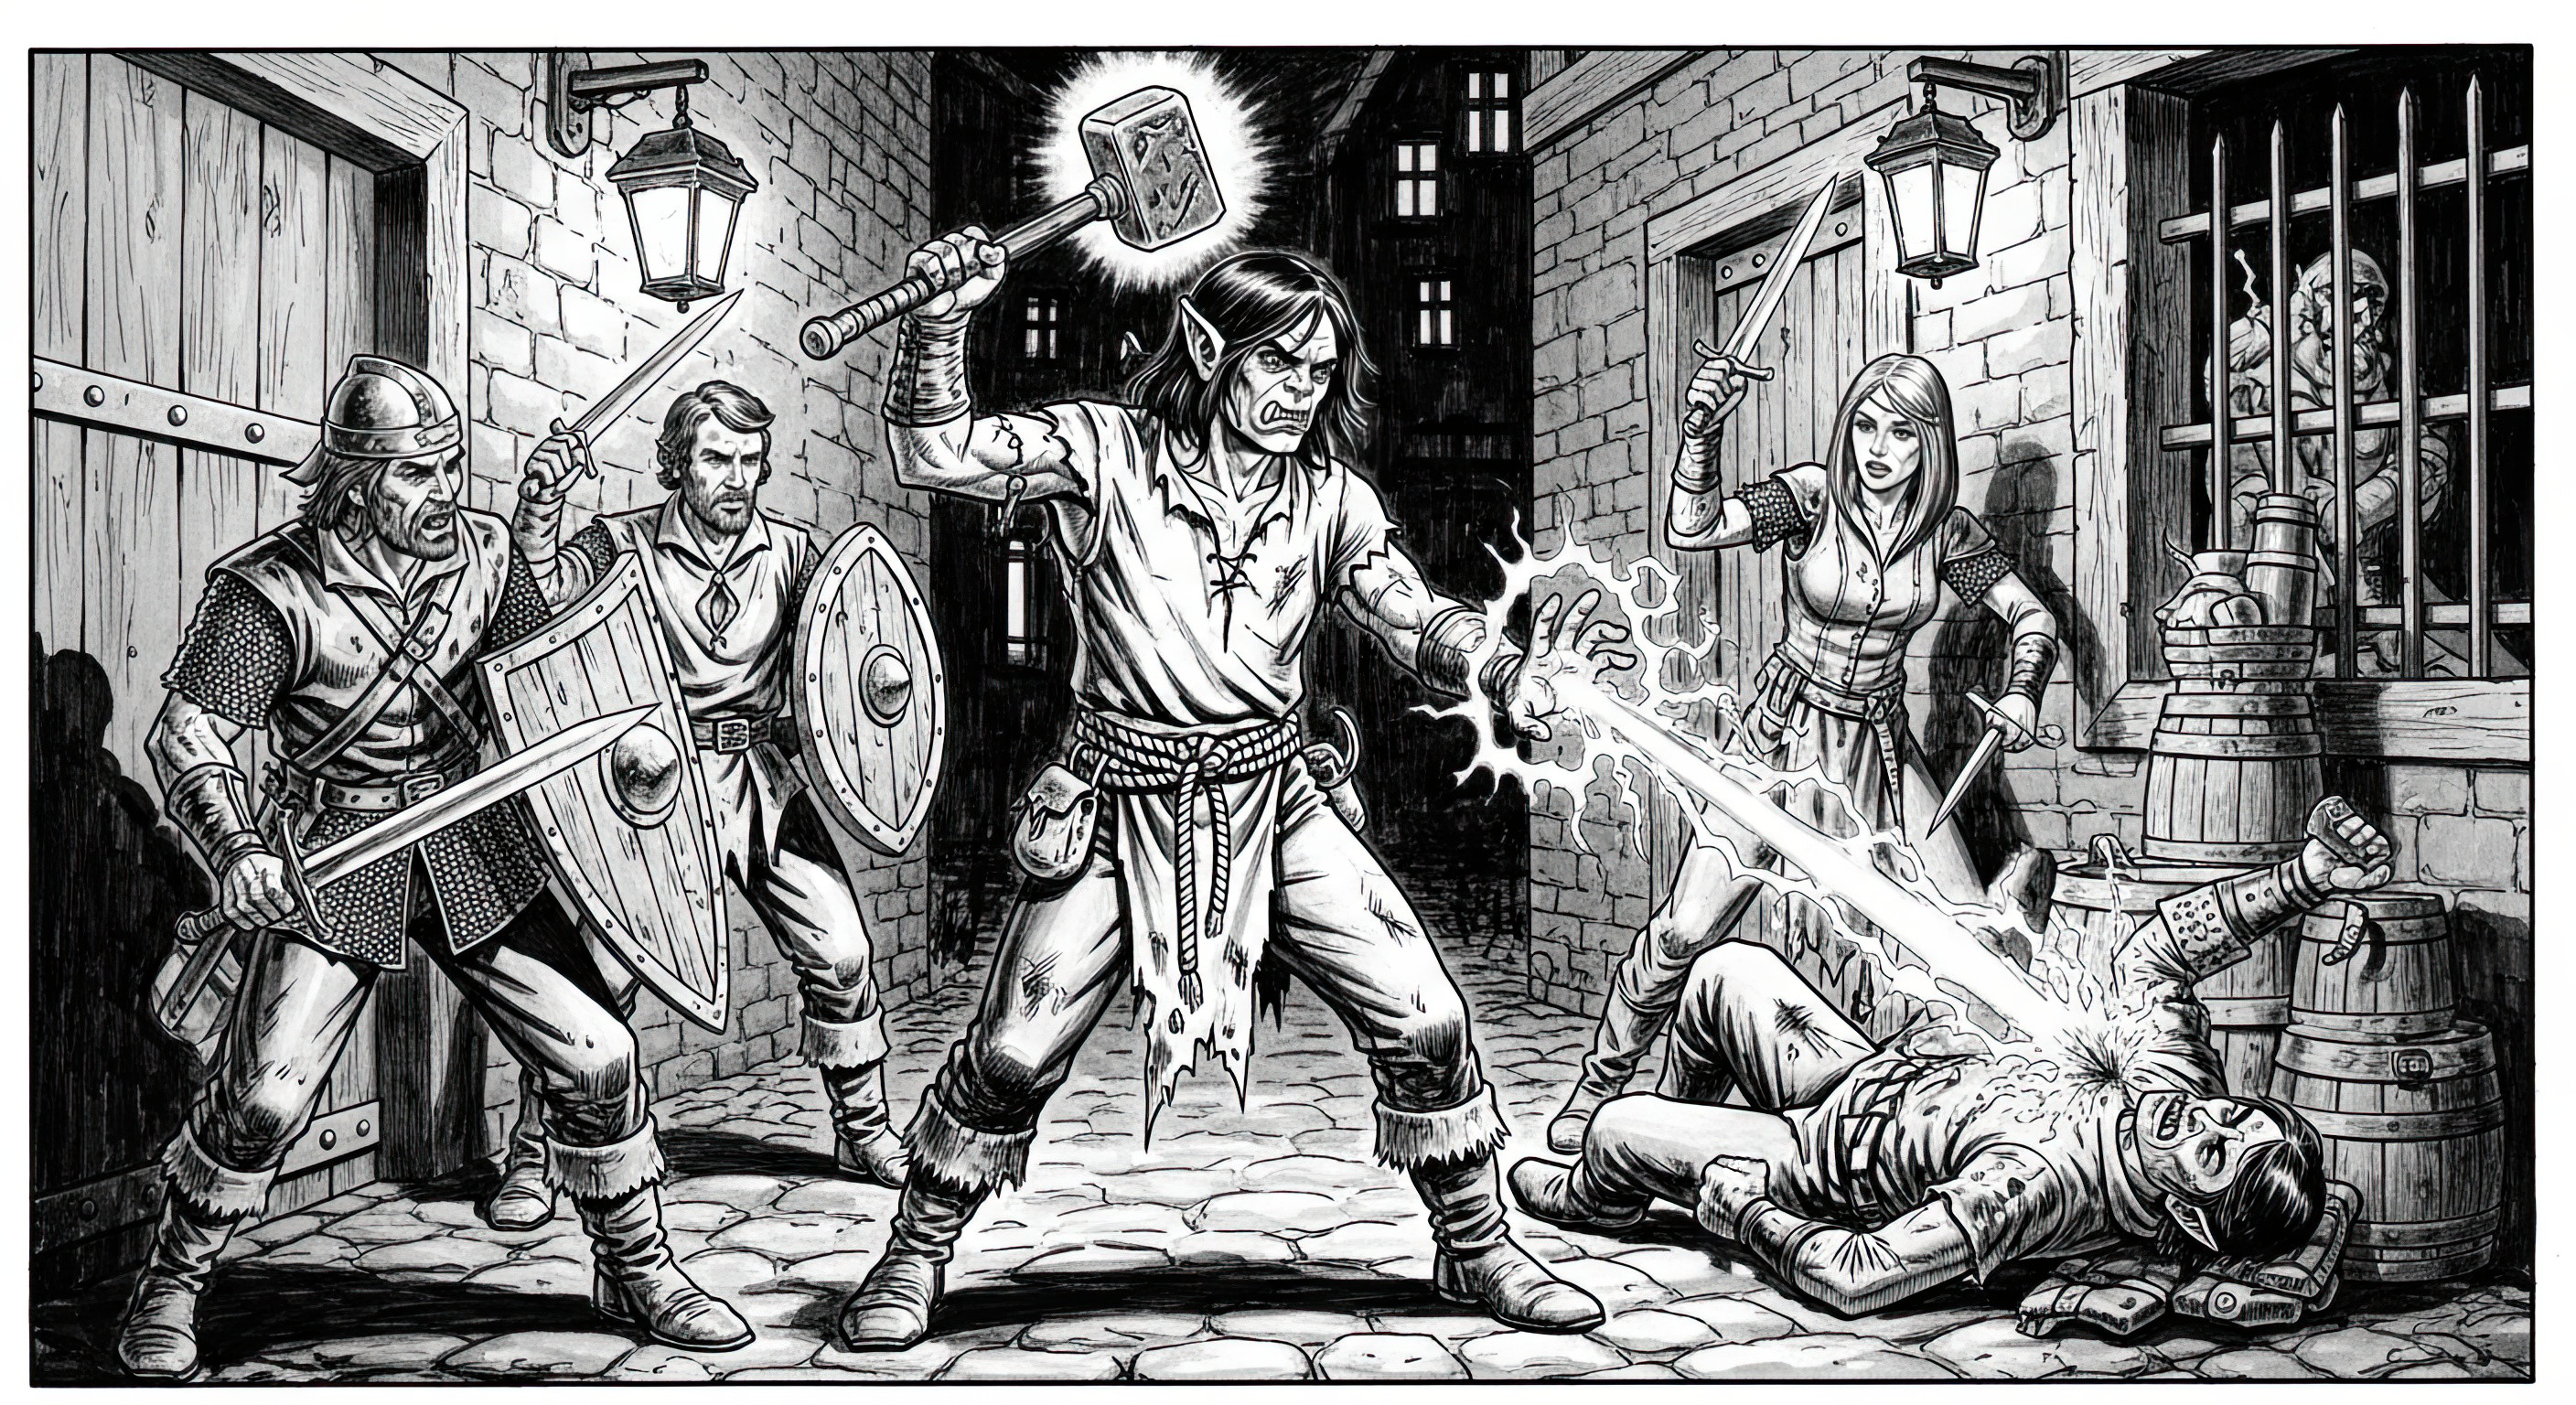
\includegraphics[keepaspectratio]{kragor-awakens.jpg}}
\end{figure*}

Since then dream visions have continued to haunt my slumber and reveal
the depth of my awakened abilities. With my war hammer raised and
eldritch energy crackling at my fingertips, I have fought against the
tyrants at every opportunity, protecting those they sought to exploit.

Gradually, my dreams began to make some sense--- as a command and as a
promise for greater power. ``Go north. Cross the frozen north. To
Eiselcross.'' The purpose remained veiled, but my resolve was absolute.
I would follow.

I traveled six weeks winding through Bladegarden, Hupperdook, Nogvugrot,
and Yrrosa, until Icehaven emerged from the frost. A Righteous Brand
veteran now seeking his own fortune was a tale that opened purses and
secured passage. Merchants, traders, wandering groups paid for my
protection, though my true purpose was survival. Traveling alone meant
certain death. Joining caravans and groups was a matter of strategic
necessity.

Dangerous encounters were rare, but not nonexistent. Most challenges I
met with cunning and bluff, my war hammer a sufficient deterrent. But
when serious threats pressed--- moments that demanded more than just
smashing some heads--- I would resort to my eldritch powers, breaking
the careful illusion of a simple veteran soldier. Sometimes those who
witnessed this would withdraw, recognizing I was something else
entirely, leaving me to continue my calculated journey north on my own.

Once I reached Icehaven I made bargain with the first captain who would
take me. The rest you know as we all met on board the \emph{Frostwind}
on our way to Palebank Village.

\chapter{Scarlet Tanager}\label{scarlet-tanager}

Scarlet Tanager grew up tangled in brambles and birdcalls, raised more
by moss and moonlight than by halfling hearths. Her early days were wild
--- tracking foxes through the fog, mimicking bird whistles, and napping
on sun-warmed roots with her owl companion Sparky perched nearby.

From the forest, she learned healing --- which roots soothed pain, which
fungus cured rot, which songs calmed frightened deer. But she also
studied: sketching leaves in a threadbare notebook, tracking lunar
cycles, deciphering glyphs etched in ancient bark.

The spirits of the land spoke to her. Not always in words, but in wind
patterns and animal eyes. When she first called one forth --- a
shimmering elk that lingered only long enough to chase away a pack of
wolves --- she knew she was not just a druid. She was a Shepherd.

She's not without flaws. Scarlet's curiosity sometimes outweighs her
caution. Her fingers tend to ``borrow'' interesting things, and while
she trusts nature implicitly, she has a harder time trusting people. But
she protects the wild and its creatures fiercely --- and now, in
Eiselcross, where magic runs old and thin beneath the ice, she listens
for the voices only she can hear.

\chapter{Whisper of Misty Valley}\label{whisper-of-misty-valley}

A tabaxi sailor turned monk, known for exceptional agility, stealth, and
scouting. She prefers claws and thrown weapons in combat, and will
choose to grapple and securely bond given the opportunity.

\end{document}
